%ब
\chapter{Results and Discussions}


The performance of the solutions while validating referential integrity in the
experiments is measured in terms of response time and throughput, which are
common \ac{DBMS} performance indicators (\todo{cite Demurjian, Berkely}).
% Response time refers to the time  a database system takes to process an
% operation and produce results to the end user and is measured without
% considering the internal functioning  of the database system (\todo{cite
% Demurjian}). This gives  details about the \ac{DBMS}
% efficiency and its speed in performing operations. 
The response time of the solutions indicate the speed with which Cassandra
completes an operation when validations are implemented.
% This included the time involved to access and retrieve metadata for the entities
% and also the time for validating referential integrity by the
% \texttt{ValidationHandler}. 
The response time of Cassandra when such validations
are not in place is also measured and considered as a baseline with which to
analyse the solutions. Such a comparison determines the degree of change in
speed of Cassandra when such additional validations are introduced and gives
 useful information about how each solution affects the performance of the
 \ac{DBMS}.

The second performance measure used is \textit{Throughput} and in the
experiments, it is measured as operations per second for all the operations
triggering referential integrity validation namely, \texttt{Create},
\texttt{Update} and \texttt{Delete}.
% A single operation
% stands for each time an entity is inserted, updated or deleted. Note that only
% the operations that introduce the referential integrity validation in Cassandra
% is measured and thus \texttt{read} operations are not measured in terms of
% response time or throughput.

% It has to be noted that the operations are prone to  external factors like
% network latency, bandwidth, network routing, network workload among others which
% typically affect a network consisting of several machines and users. This is
% because the Cassandra cluster used in the experiments is deployed over a
% network that is used by many users concurrently thus exposing the operations to
% such factors. Identifying such factors and analysing them is beyond the scope of
% this thesis and the analysis is strictly in terms of how the metadata storage
% and referential integrity validation affects Cassandra's performance.

 The results from the experiments were used to
analyse the performance of the four solutions  and this is discussed in the
following sections.
Section~\ref{s:results-overview} presents the overall performance of the four
solutions in the experiment.
Section~\ref{s:results-Baseline} presents the results for the baseline
experiment.
Section~\ref{s:results-insert} analyses the results of all the solutions for the
\texttt{insert} operation.
Section~\ref{s:results-update} presents the analysis for the \texttt{update}
operation for all the solutions.
Section~\ref{s:results-Delete} discusses the results of the solutions for the
\texttt{delete} operation.
Section~\ref{s:results-summary} summarises the analysis of the results of all
the solutions.

\newcommand{\Width}{0.5\textwidth}
\newcommand{\TB}[1]{\textbf{#1}}

\section{Overview of Results} \label{s:results-overview}

The experiments were run with the objective of measuring the performance of the
solutions and to determine how the metadata storage and validations in each
solution affects the performance of Cassandra. The results from these
experiments are presented in
Tables~\ref{tres:ResponseTime},~\ref{tres:ResponsetimeRatio},~\ref{tres:Throughput}
and~\ref{tres:ThroughputRatio}. 

Table~\ref{tres:ResponseTime} presents the response time (in milliseconds) of
all the solutions and shows the amount of time taken to complete one operation
on each entity.
Table~\ref{tres:Throughput} shows the throughput of each operation on an entity,
that is, how many operations can be completed on an entity in one second.
Table~\ref{tres:ResponsetimeRatio} shows the ratio of the response time of each
solution when compared to the response time of the baseline and indicates
how many times faster or slower each solution is when compared to the baseline.
Similarly, Table~\ref{tres:ThroughputRatio} shows the ratio of the throughput of
the solutions when compared to the throughput of the baseline. 

As seen in these results, Solution~4 performs the best amongst all the solutions
since the response times for all the  operations on every entity are the least
for Solution~4. Note that these values are higher than the response times for
Baseline  because the baseline does not perform any referential
validations or store metadata. Solution~3 performs the worst amongst all the
solutions with high response times for all the operations and the least
throughput in all the cases. Solutions~1 and 2 perform similarly, although
Solution~1 is faster with slightly lesser response times.

% The results show the throughput and the response time
% of each solution to complete an operation with referential integrity validation
% on a single entity. The throughput shows how many operations are performed in
% one second in each solution. The solution with the lowest response time and
% highest throughput shows its faster in performing the operations.

The results show that all the solutions perform differently and have different
response times and throughput. The variations in  performance of the solutions
is due to the different ways of storing  metadata in each solution. Recall that
Solutions~1 and 2 save metadata along with the entity where Solution~1 stores it
in every row and Solution~2 stores it in the top row of a column family. On the
other hand, Solutions~3 and 4 store metadata separate from the actual data  in a
separate \texttt{Metadata} column family but Solution~4 stores the
\texttt{Metadata} column family in a separate cluster. The way metadata is
stored and retrieved in each solution affects its performance during validation,
when constraints are retrieved and used as explained in Chapter~\ref{c:Implementation}.

Solution~4  is faster than the other solutions to perform the validations on
each operation because it caches the list of constraints and avoids connecting
to the external cluster to access the \texttt{Metadata} column family each time
an operation is invoked. Therefore, to locate the relevant \ac{FK} and \ac{PK}
constraints of an entity, the constraints stored in the cache are re-used.
Performance is improved by caching the entire \texttt{Metadata} column family
and and saves time by reducing the number of times a separate column family has
to be accessed each time to complete a validation.

Solution~3 is the slowest among the solutions because of the way it accesses the
metadata.
% of the way the metadata is accessed for the entities in this solution.
% % irrespective of whether an entity is a parent or child the %
% \texttt{ValidationHandler} performs the same check the metedata of the entity
% % for all the solutions. It is when this check is made it is clear if the
% entity % is a parent or child.
% In this solution accessing
In this solution, in order to retrieve the relevant \ac{FK} constraints for
every entity the \texttt{Metadata} column family has to be accessed. This means
that for each operation on an entity, \texttt{Metadata} is accessed using the
connection object which consumes more time to complete the operation. Moreover,
to retrieve information about any referencing constraints within the relevant
\ac{FK} constraints, \texttt{Metadata} is accessed again. For example, in
order to get the information of a \ac{PK} constraint stored in the
\texttt{RConstraintName} column of a \ac{FK} constraint, the \texttt{Metadata}
column family is again accessed and the \ac{PK} constraint is searched. Thus to
complete each validation, \texttt{Metadata} is accessed more than once.
% \texttt{Metadata} column family has to be accessed using the connection
% object.
This is because metadata is not cached for re-use in this solution, unlike
Solution~4 costing multiple column family access.

Solutions~1 and~2 have approximately similar response times. Both the solutions
store the list of constraints as a part of the entity and accessing the relevant
constraints or referenced constraints of an entity requires no additional
connections to another column family. Since the constraints are stored with the
entity in both these solutions, a cache to store the metadata is not required.
Note that Solution~1 performs marginally better than Solution~2 
because Solution~2 has an additional search operation to identify the top row in a
column family to locate the relevant constraints of an entity.
% their metadata access for these solutions are easier as metadata is a part of
% the entity and no additional connection to a metadata column family is
% required.


% Unlike this, Solution~4 caches  metadata for entities and re-uses it thus
% saving time by not having to access a separate column family for each entity
% insertion.

The performance of the solutions in each
operation on the entities is discussed in detail in the following sections.
 %ब 

\newcolumntype{B}{>{\columncolor{light-gray}}c} 

	\begin{table}[t]
	\renewcommand*\arraystretch{1}
	
% 	\newcolumntype{C}{@{\hspace{3pt}}>{\scriptsize}c@{\hspace{3pt}}}
	\newcolumntype{C}{c}
	\footnotesize
% 	\small
	\centering
	\caption{Response time in milliseconds per entity}\label{tres:ResponseTime}
		\begin{tabular}{CCBCCCC}
		
			\toprule &&\textbf{Baseline} & \textbf{Solution1} & \textbf{Solution2} &
			\textbf{Solution3} & \textbf{Solution4}\\
						
			\midrule \multirow{3}{*}{\textbf{insert}} & \textbf{s} & 0.366 (0.08) & 0.568
			(0.03) & 0.820 (0.09) & 2.108 (0.05) & \TB{0.364 (0.02)}\\
			& \textbf{c} & 0.352 (0.05) & 0.547 (0.04) & 0.803 (0.05) & 2.092 (0.06) &
			\TB{0.351 (0.01)}\\
			& \textbf{e} & 0.305 (0.01) & 1.239 (0.04) & 1.405 (0.02) & 3.484 (0.05) &
			\TB{0.936 (0.01)}\\
						
			\midrule \multirow{3}{*}{\textbf{update}} & \textbf{s} & 0.730 (0.16) & 19.144
			(0.39) & 20.840 (0.43) & 46.394 (0.73) & \TB{14.997 (0.37)}\\
			& \textbf{c} & 0.759 (0.06) & 5.810 (0.50) & 5.991 (0.27) & 10.419 (0.30)
			& \TB{4.751 (0.28)}\\
			& \textbf{e} & 0.404 (0.03) & 1.353 (0.03) & 1.500 (0.02) & 3.579 (0.05) &
			\TB{1.031 (0.01)}\\
						
			\midrule \multirow{3}{*}{\textbf{delete}} & \textbf{s} & 0.314 (0.03) & 7.425
			(0.44) & 10.533 (0.41) & 26.023 (0.55) & \TB{5.638 (0.37)}\\
			& \textbf{c} & 0.287 (0.05) & 2.037 (0.08) & 2.367 (0.09) & 3.958 (0.12) &
			\TB{1.964 (0.09)}\\
			& \textbf{e} & 0.290 (0.03) & 0.410 (0.02) & 0.744 (0.02) & 2.132 (0.04)
			& \TB{0.299 (0.02)}\\
						
			\bottomrule
		\end{tabular}
	\vspace{1cm}
	\captionof{table}{Response time ratio with respect to
	Baseline}\label{tres:ResponsetimeRatio}
		\begin{tabular}{cccccc}
			 
			\toprule && \textbf{Solution1} & \textbf{Solution2} &
			\textbf{Solution3} & \textbf{Solution4}\\
						
			\midrule \multirow{3}{*}{\textbf{insert}} & \textbf{s} & 1.55 & 2.24 &
			5.76 & \TB{0.99}\\
			& \textbf{c} & 1.56 & 2.28 & 5.95 & \TB{1.00}\\
			& \textbf{e} & 4.06 & 4.61 & 11.42 & \TB{3.07}\\
						
			\midrule \multirow{3}{*}{\textbf{update}} & \textbf{s} & 26.21 & 28.53 &
			63.51 & \TB{20.53}\\
			& \textbf{c} & 7.66 & 7.90 & 13.74 & \TB{6.26}\\
			& \textbf{e} & 3.35 & 3.71 & 8.86 & \TB{2.55}\\
						
			\midrule \multirow{3}{*}{\textbf{delete}} & \textbf{s} & 23.61 & 33.50 &
			82.76 & \TB{17.93}\\
			& \textbf{c} & 7.09 & 8.24 & 13.78 & \TB{6.84}\\
			& \textbf{e} & 1.41 & 2.57 & 7.36 & \TB{1.03}\\
			
			\bottomrule
%  			\multicolumn{3}{l}{}%\scriptsize $^*$ Milliseconds per entity} 
 			
			\multicolumn{6}{r}{\scriptsize Lower values mean faster response}
		
		\end{tabular}
	\end{table}
	
	\begin{table}[t]
	\renewcommand*\arraystretch{.9}
	\footnotesize
% 	\small
	\centering
	\caption{Throughput in entities per second}\label{tres:Throughput}
		\begin{tabular}{ccBcccc}
			
			\toprule
			&&\textbf{Baseline} & \textbf{Solution1} & \textbf{Solution2} &
			\textbf{Solution3} & \textbf{Solution4}\\
			
			\midrule \multirow{3}{*}{\textbf{insert}} & \textbf{s} & 2790 (291) & 1764 (85)
			& 1228 (82) & 475 (12) & \TB{2755 (125)}\\
			& \textbf{c} & 2880 (264) & 1837 (112) & 1250 (69) & 478 (13) & \TB{2856
			(96)}\\
			& \textbf{e} & 3282 (116) & 807 (22) & 712 (11) & 287 (4) & \TB{1069 (15)}\\
			
			\midrule \multirow{3}{*}{\textbf{update}} & \textbf{s} & 1394 (121) & 52 (1) &
			48 (1) & 22 (0) & \TB{67 (2)}\\
			& \textbf{c} & 1325 (97) & 173 (14) & 167 (7) & 96 (3) & \TB{211 (12)}\\
			& \textbf{e} & 2483 (119) & 739 (15) & 667 (11) & 279 (4) & \TB{970 (12)}\\
			
			\midrule \multirow{3}{*}{\textbf{delete}} & \textbf{s} & 3198 (205) & 135 (8) &
			95 (4) & 38 (1) & \TB{178 (11)}\\
			& \textbf{c} & 3574 (567) & 492 (19) & 423 (15) & 253 (7) & \TB{510 (21)}\\
			& \textbf{e} & 3470 (206) & 2443 (95) & 1346 (44) & 469 (9) & \TB{3351
			(167)}\\
			\bottomrule
		\end{tabular}

	\vspace{1cm}
	
	\captionof{table}{Throughput ratio with respect to Baseline}
	\label{tres:ThroughputRatio}
		\begin{tabular}{cccccc}
			
			\toprule
			&&\textbf{Solution1} & \textbf{Solution2} &
			\textbf{Solution3} & \textbf{Solution4}\\
			
			\midrule
			\multirow{3}{*}{\textbf{insert}} & \textbf{s} & 0.63 & 0.44 & 0.17 &
			\TB{0.99}\\
			 & \textbf{c} & 0.64 & 0.43 & 0.17 & \TB{0.99}\\
			 & \textbf{e} & 0.25 & 0.22 & 0.09 & \TB{0.33}\\
			
			\midrule
			\multirow{3}{*}{\textbf{update}} & \textbf{s} & 0.04 & 0.03 & 0.02 &
			\TB{0.05}\\
			 & \textbf{c} & 0.13 & 0.13 & 0.07 & \TB{0.16}\\
			 & \textbf{e} & 0.30 & 0.27 & 0.11 & \TB{0.39}\\
			
			\midrule
			\multirow{3}{*}{\textbf{delete}} & \textbf{s} & 0.04 & 0.03 & 0.01 &
			\TB{0.06}\\
			 & \textbf{c} & 0.14 & 0.12 & 0.07 & \TB{0.14}\\
			 & \textbf{e} & 0.70 & 0.39 & 0.14 & \TB{0.97}\\
			
			\bottomrule
% 			\scriptsize $^*$ Entities per second
% 			\multicolumn{3}{l}{} & &
			\multicolumn{6}{r}{\scriptsize Higher values mean more throughput}
		\end{tabular}
	\end{table}







\section{Baseline Operations} \label{s:results-Baseline}

The performance of Cassandra when referential
integrity validations are introduced  is compared with
 a base experiment where the operations on the entities do not trigger any
such validations. Such a baseline serves as a reference to determine the
difference in performance of the \ac{DBMS} when validations are imposed using
the \ac{API} and to analyse the performance of the solutions.

In the baseline experiment, the operations on the entities represent how data is
inserted into Cassandra, i.e. without referential integrity validations.
The results in terms of response time and throughput for the baseline experiment
is presented as  bar-plots in Figure~\ref{fres:Baseline}.
Figure~\ref{fres:Baseline-responsetime} shows the response time (in
milliseconds) of each operation on a single entity of the three column families.
Figure~\ref{fres:Baseline-throughput} presents the throughput of each operation
on the three column families in one second. 
% The analysis of the performance of
% each operation on an entity is discussed as follows.

% 	\begin{figure}[h] \centering
% 	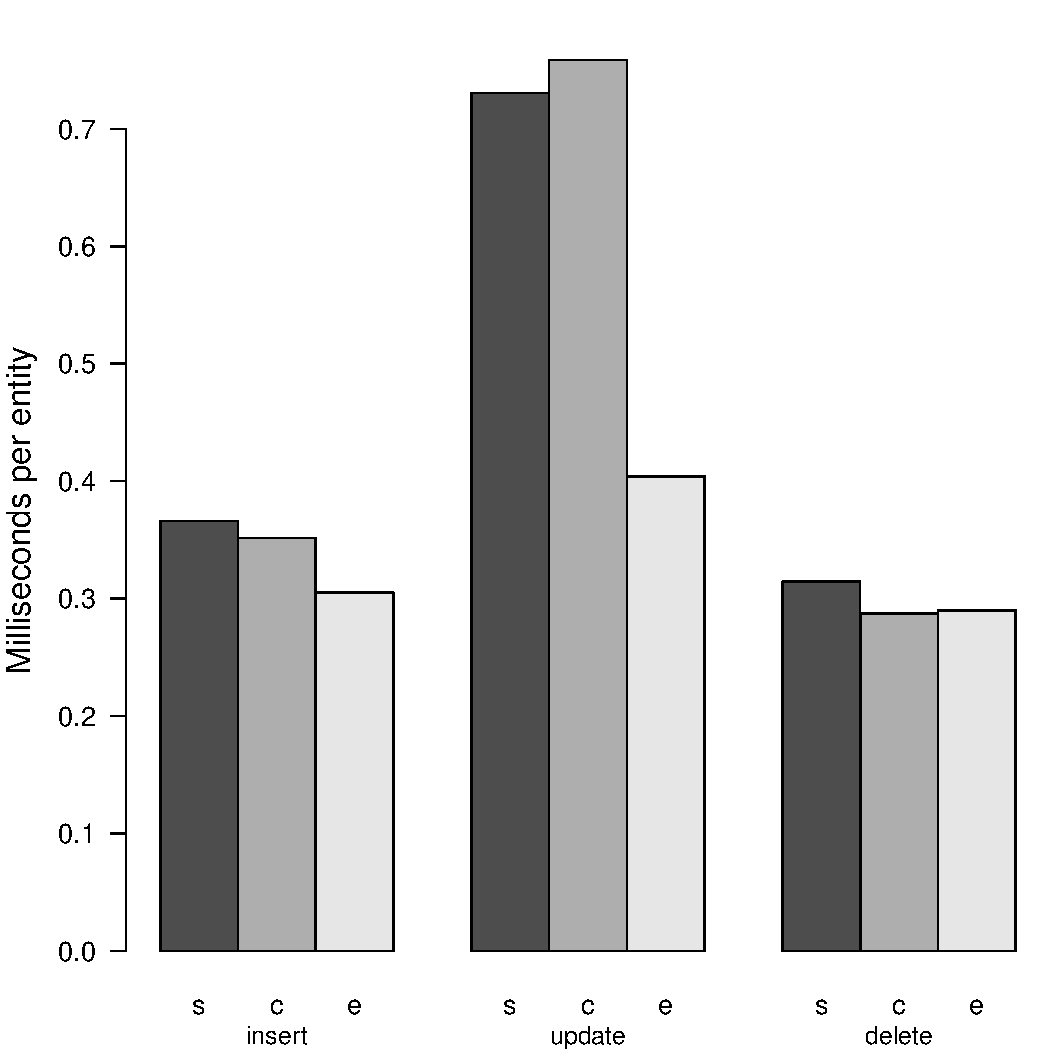
\includegraphics[width=.8\textwidth]{./figure/result/barplot-Baseline-rt.pdf}
% 		\caption{Baseline}\label{fr:Solution0-barplot}
% 	\end{figure}
	
	\begin{figure}[H]
		
		\subfigure[Response time for Baseline]
		{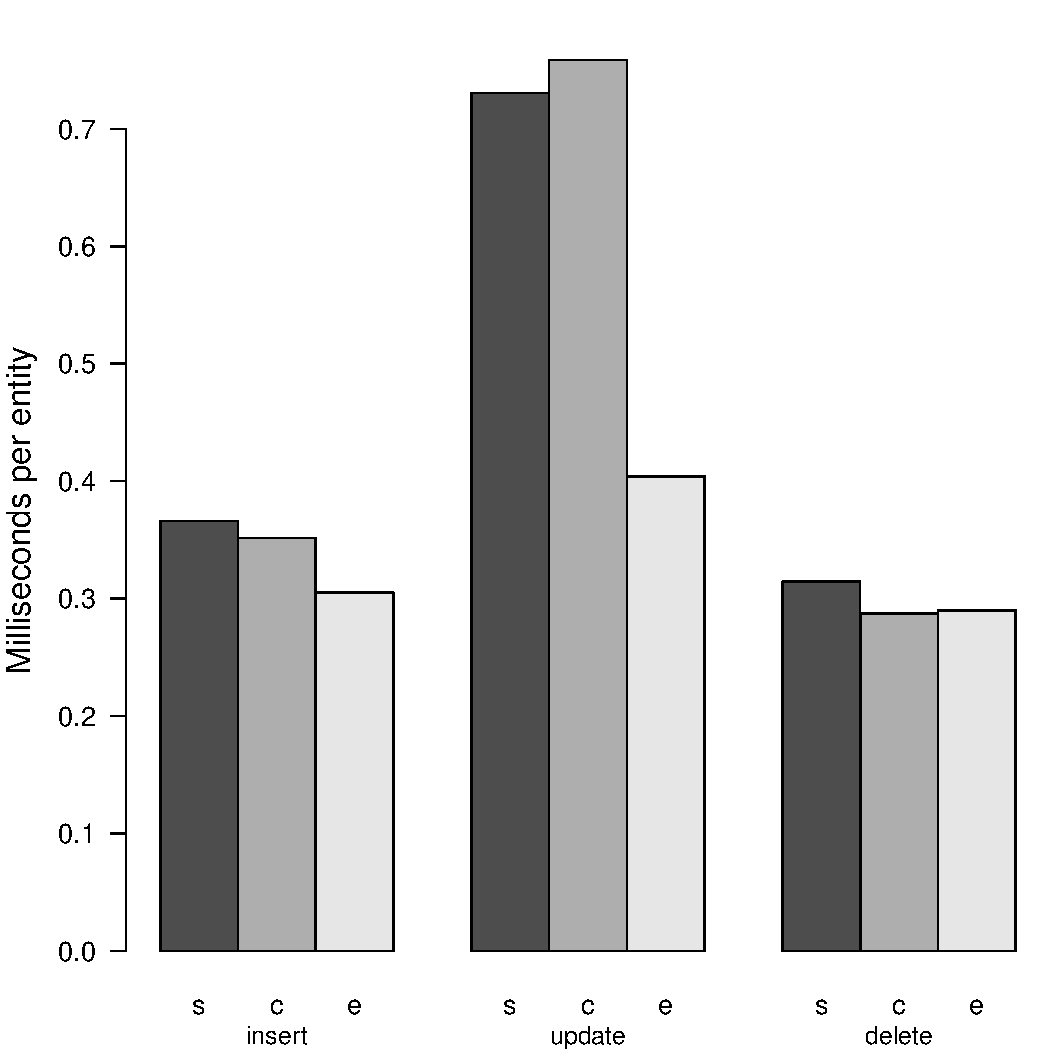
\includegraphics[width=\Width]{figure/result/barplot-Baseline-rt.pdf}\label{fres:Baseline-responsetime}}
		\subfigure[Throughput for Baseline]
		{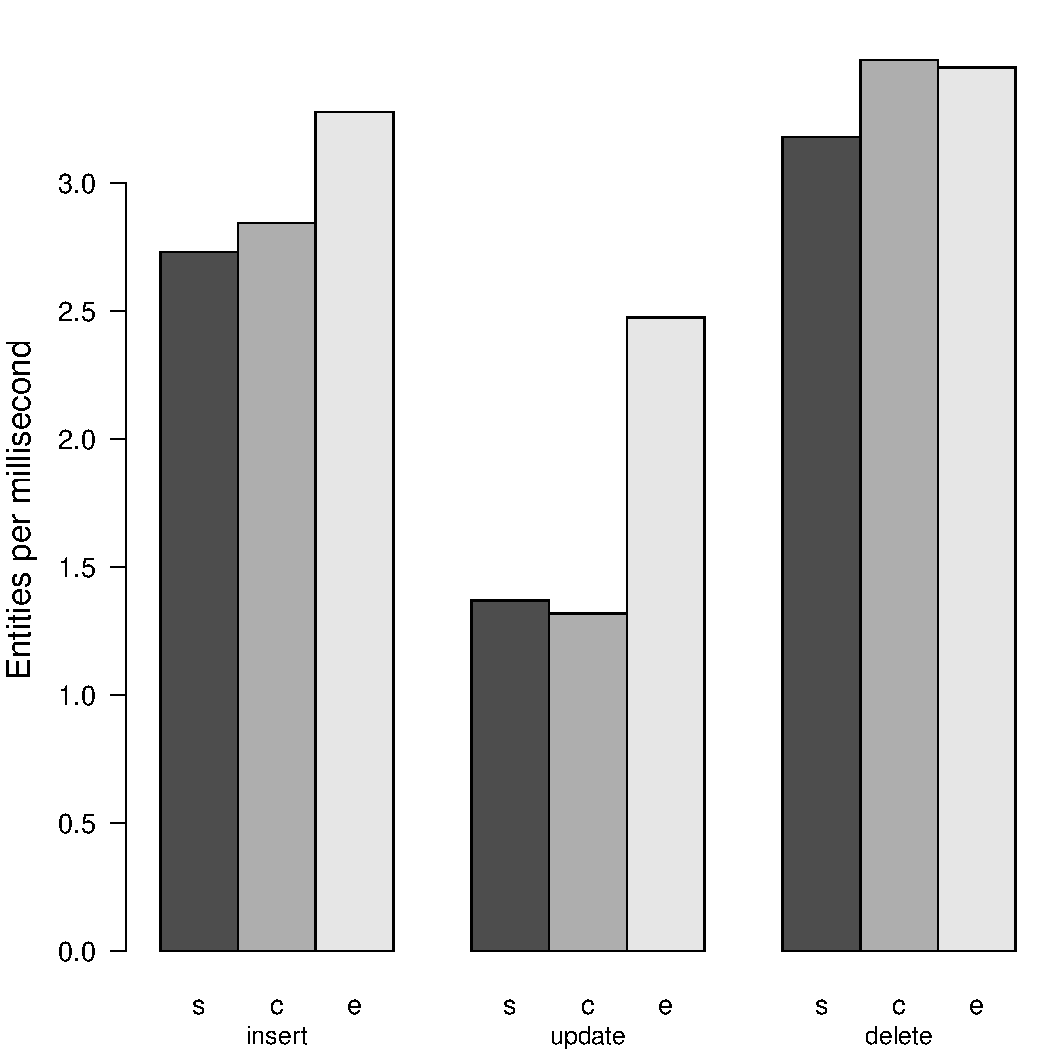
\includegraphics[width=\Width]{figure/result/barplot-Baseline-tp.pdf}\label{fres:Baseline-throughput}}
		\caption{Performance of Baseline}\label{fres:Baseline}
	\end{figure}

As seen from these results, \texttt{Delete} operation takes the least response
time and has the highest throughput. That is, the time to delete an entity is
lesser when compared to \texttt{Insert} and \texttt{Update} which means more
\texttt{Delete} operations are performed in a second. On the other
hand,\texttt{Update} takes the most time to complete all the operations and has
the least throughput. \texttt{Insert} takes slightly more time to complete on
all the entities than \texttt{Delete} but is faster than \texttt{Update}.

\texttt{Delete} performs faster than the other operations because Cassandra
performs a tombstone delete, where data is not immediately deleted but only
marked as deleted and maintained for the duration specified by the application
(\todo{cite book}).\texttt{update} takes the most time because it requires
searching by index to access the correct columns in the column family to write
the new value and once the correct columns are identified, the old values are
deleted and the new values are inserted. Thus, to complete an \texttt{update}, a
\texttt{delete} and an \texttt{insert} has to be performed, thus taking more
time than both \texttt{delete} and \texttt{insert}. \texttt{insert} takes
slightly more time since data is immediately written into the column
families.

The time taken to insert one entity of \texttt{Student}, \texttt{Course} and
\texttt{Enrolment} are similar since there are no additional validations or
operations to insert these entities. Note that the slight variations in the
response times for an \texttt{insert} on the entities of \texttt{Student},
\texttt{Course} and \texttt{Enrolment}is possibly due to external factors.
Moreover, when the experiments are run \texttt{insert} on these entities are the
first operations to take place and the results can be slightly influenced by the
initialisation of the column families and the keyspace. However, the difference
is small and only a fraction of a millisecond.

Note that the \texttt{Update} in \texttt{Enrolment} takes lesser time because
the number of columns  that are updated in \texttt{Enrolment} is much lesser
than the other column families. This means that \texttt{Update} on
\texttt{Enrolment} involves fewer search by indexes and writes for the new
values, to be precise it involves only three searches and writes 
to update its three columns.  On the other hand, \texttt{Student} and
\texttt{Course} column families have more number of columns to be updated in
each \texttt{Update} operation.

%ब 
\section{Insert} \label{s:results-insert}
% \newcommand{\Width}{0.5\textwidth}
% \newcommand{\TB}[1]{\textbf{#1}}
% An \texttt{insert} operation triggers a referential integrity validation
% whenever a child entity containing foreign keys is inserted where the
% \texttt{ValidationHandler} validates that the foreign keys exist as primary keys
% in the parent entities.
Across all the solutions in the experiments,  \texttt{insert}  triggers a
validation when \texttt{Enrolment} entities are inserted as it is a child entity
containing foreign keys of \texttt{Student} and \texttt{Course} entities.
\texttt{Student} and \texttt{Course} entities do not trigger validations as
these do not contain any references to other column families. 

The response time and throughput for completing an \texttt{insert} on a single
entity for all the solutions are presented in Figure~\ref{fres:Insert}.
Figure~\ref{fres:Insert-responsetime} shows the time consumed by each solution
to complete one \texttt{insert} operation in each of the three entities.
Figure~\ref{fres:Insert-throughput} shows the number of \texttt{insert}
operations that can be completed in one second across the solutions.

	\begin{figure}[H] 
		\subfigure[Response time for Insert operation]
		{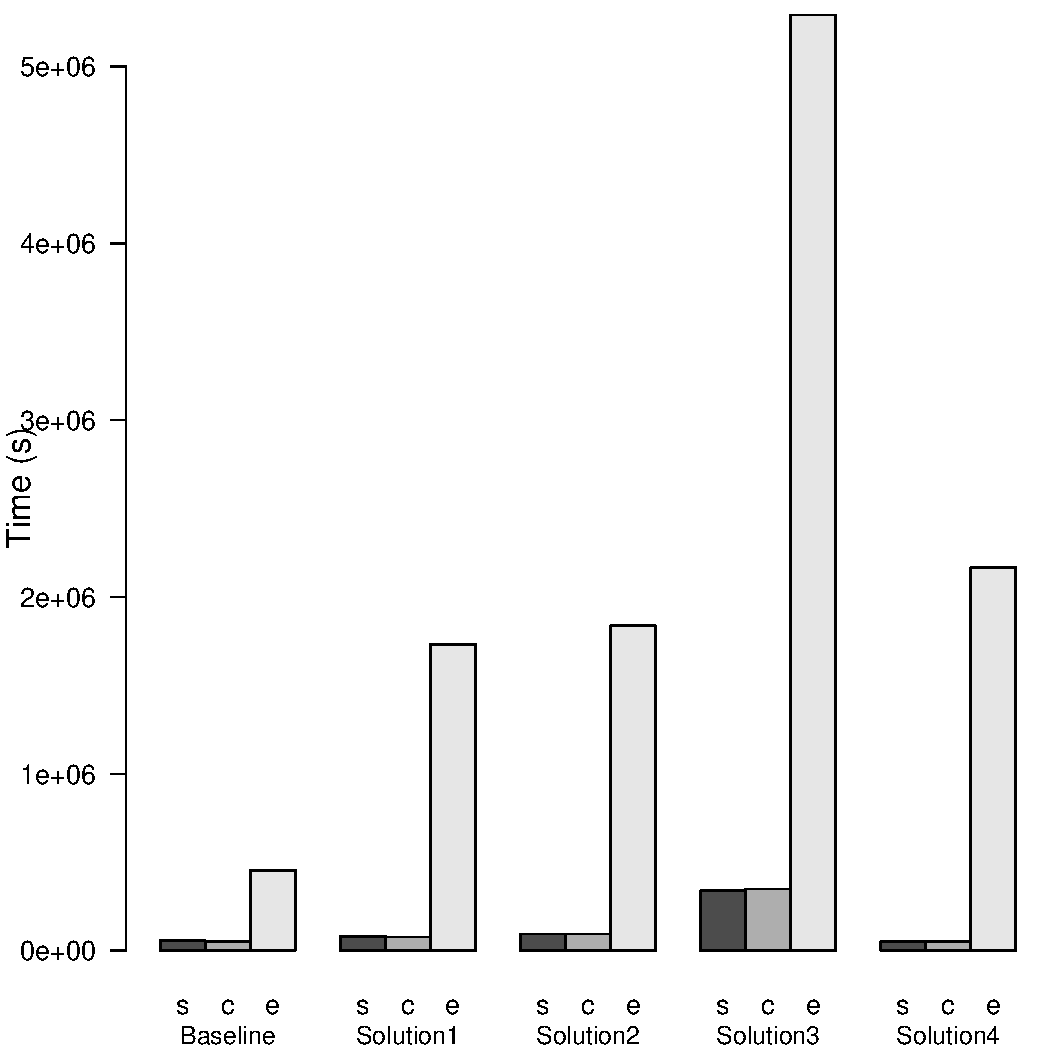
\includegraphics[width=\Width]{figure/result/barplot-insert-rt.pdf}\label{fres:Insert-responsetime}}
		\subfigure[Throughput for Insert operation]
		{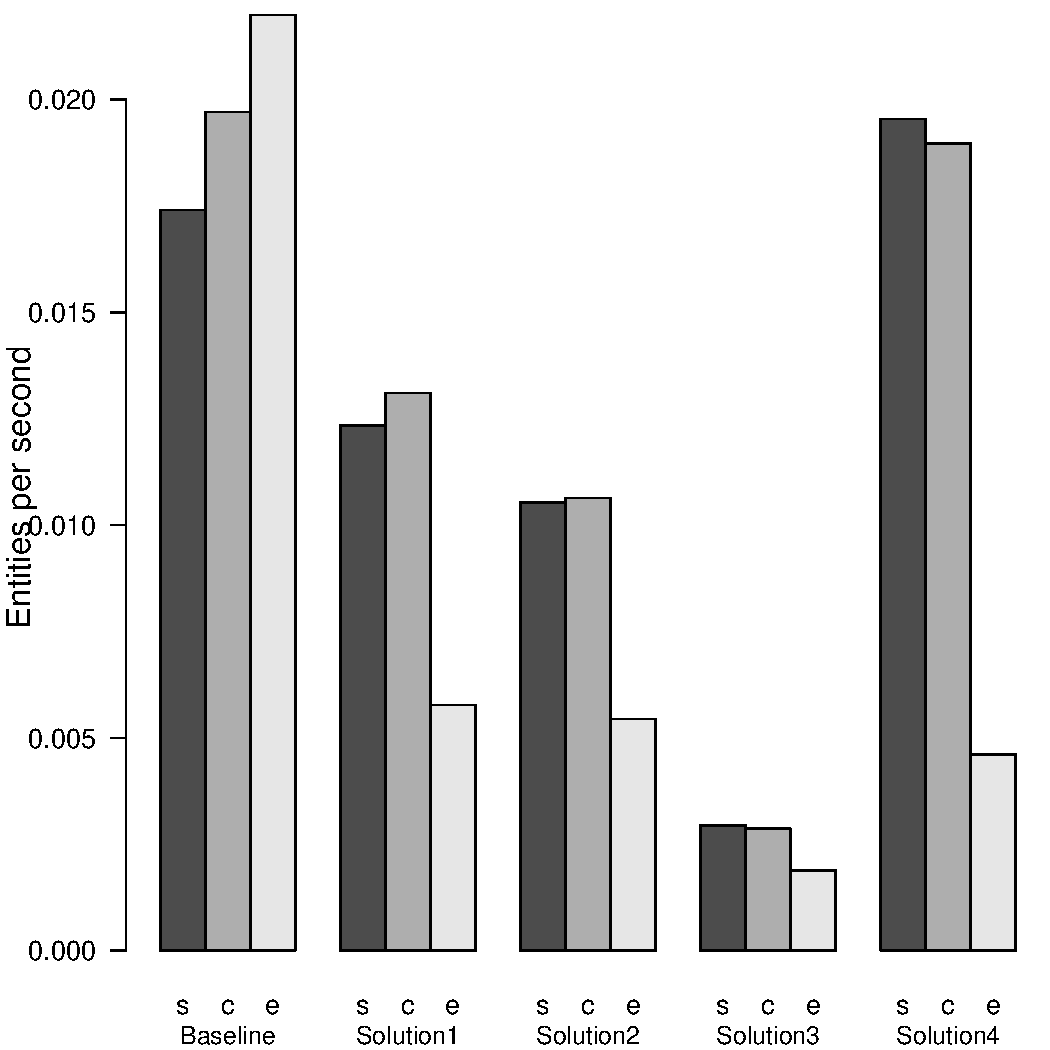
\includegraphics[width=\Width]{figure/result/barplot-insert-tp.pdf}\label{fres:Insert-throughput}}
		\caption{Performance of Solutions in Insert}\label{fres:Insert}
	\end{figure}
	
These results show
% and the results in Figures~\ref{fres:insert-user} and~\ref{fres:insert-course}
that \texttt{insert} on a single entity of \texttt{Student} and \texttt{Course}
take approximately the same time to complete. On the other hand, \texttt{insert}
on a single \texttt{Enrolment} entity takes the most time in all the solutions.
Inserting \texttt{Student} and \texttt{Course} entities into their respective
column families is fastest as these are parent column families and do not
trigger any validation. \texttt{insert} on these entities involves only
accessing its relevant \ac{FK} constraints from the metadata in order to
determine whether it is a parent or child entity. If the entity is a parent, the
validations are not triggered which is the case for \texttt{Student} and
\texttt{Course} entities. However, \texttt{Enrolment} entities have existing
\ac{FK} constraints indicating that they reference a parent entity which in turn
triggers referential integrity validations. Therefore,  its
validation involves not only identifying its relevant constraints but also
accessing its parent column families \texttt{Student} and \texttt{Course} to
ensure the existence of the foreign keys.
The results highlight the difference in response time when validation is
triggered in the case of \texttt{Enrolment} as well as when it is not initiated
in the parent entities.
% the validation of one \texttt{Enrolment} entity and for other entities that do
% not have validations.
Note that these observations stand true across all the solutions.

More information about the performance of each solution when an \texttt{insert}
operation is executed on each entity is presented in
Figures~\ref{fres:insert-user},~\ref{fres:insert-course}
and~\ref{fres:insert-enrolment}.
These figures show the response time for one \texttt{insert}
on all the three entities in every solution and the throughput for the
operations.
Figure~\ref{fres:insert-user} presents the results for \texttt{insert} on a
single \texttt{Student} entity in all the solutions. Similarly
Figures~\ref{fres:insert-course} and~\ref{fres:insert-enrolment} show the
performance of \texttt{insert} on a \texttt{Course} and \texttt{Enrolment}
entity in the solutions. It can be seen that Solution~4 takes the least time to
complete an \texttt{insert} on all the entities while Solution~3 takes the most
time. Both Solutions~1 and 2 perform similarly and are slightly slower than
Solution~4. These differences are because of the way their metadata is stored
and accessed as explained in Section~\ref{s:results-overview}.

When compared to the baseline, it is clear that the referential integrity
validations as well as metadata access caused the increased response time for
\texttt{insert} in all the solutions. Since the validations are the same for all
solutions, the performance differences in the solutions are due to the different
ways of accessing and processing the metadata.
Solution~4 is almost three times slower than the baseline to perform the
validations on \texttt{insert} while Solution~3 is more than eleven times
slower. Both Solutions~1 and 2 are almost four times slower than the baseline.
% Solution~3 takes the most time to perform one \texttt{insert} on all the
% entities.
However, when no validations are triggered Solution~4 performs almost similar to
the baseline while Solution~3 is still about two times slower than the baseline.
In this case, Solutions~1 and 2 are only about 0.5 times slower than the
baseline. Note that the time to \texttt{insert} \texttt{Student} and
\texttt{Course} entities in Baseline and Solution~4 are similar (Figures~\ref{fres:insert-user}
and~\ref{fres:insert-course}). A possible reason for this is that baseline
operations are affected by the initialization as its \texttt{insert} operations
are the very first operations to be executed.

\newpage
		\begin{figure}[H]
		\centering
		\newcommand{\W}{.4\textwidth}
			\subfigure[Response time for Insert on Student]
			{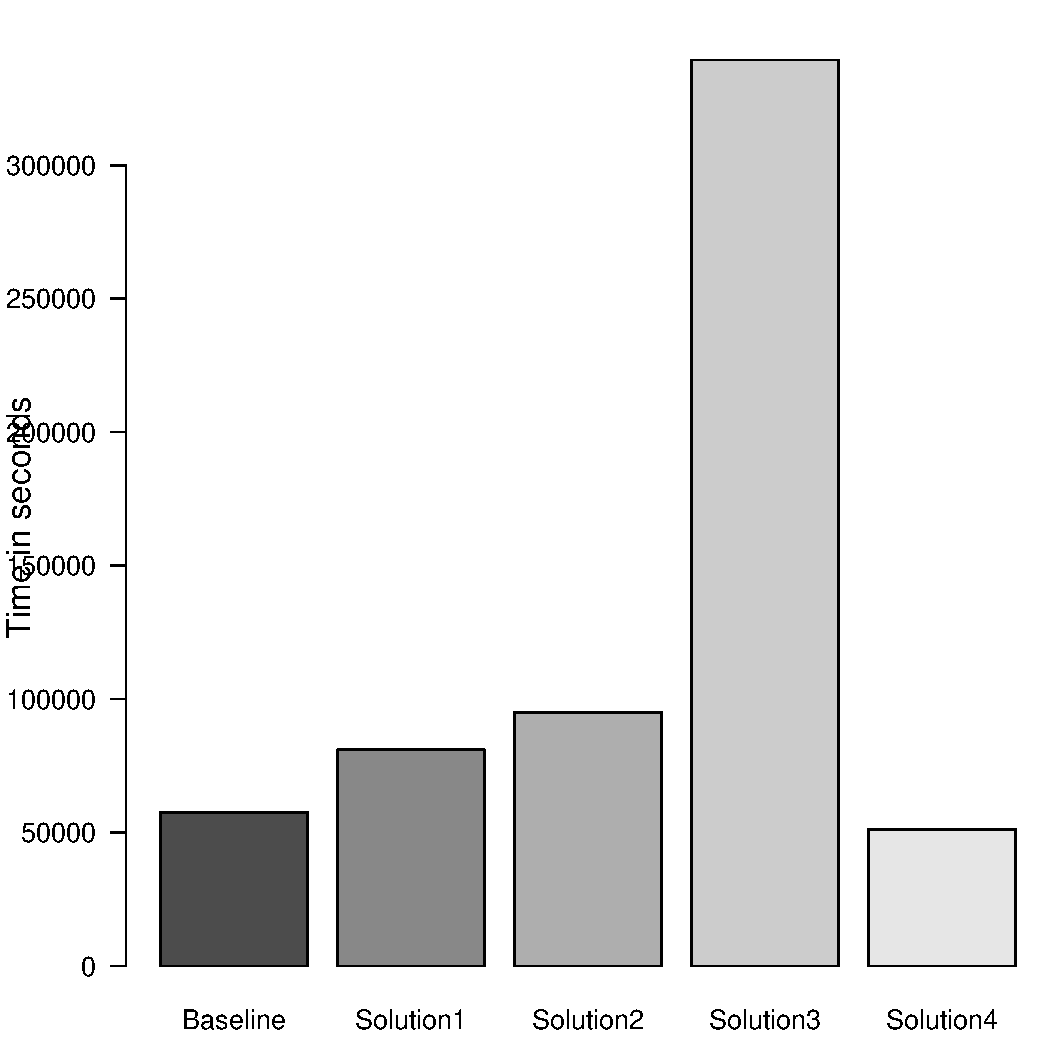
\includegraphics[width=\W]{figure/result/barplot-insert_student-rt.pdf}}
			\subfigure[Throughput for Insert on Student]
			{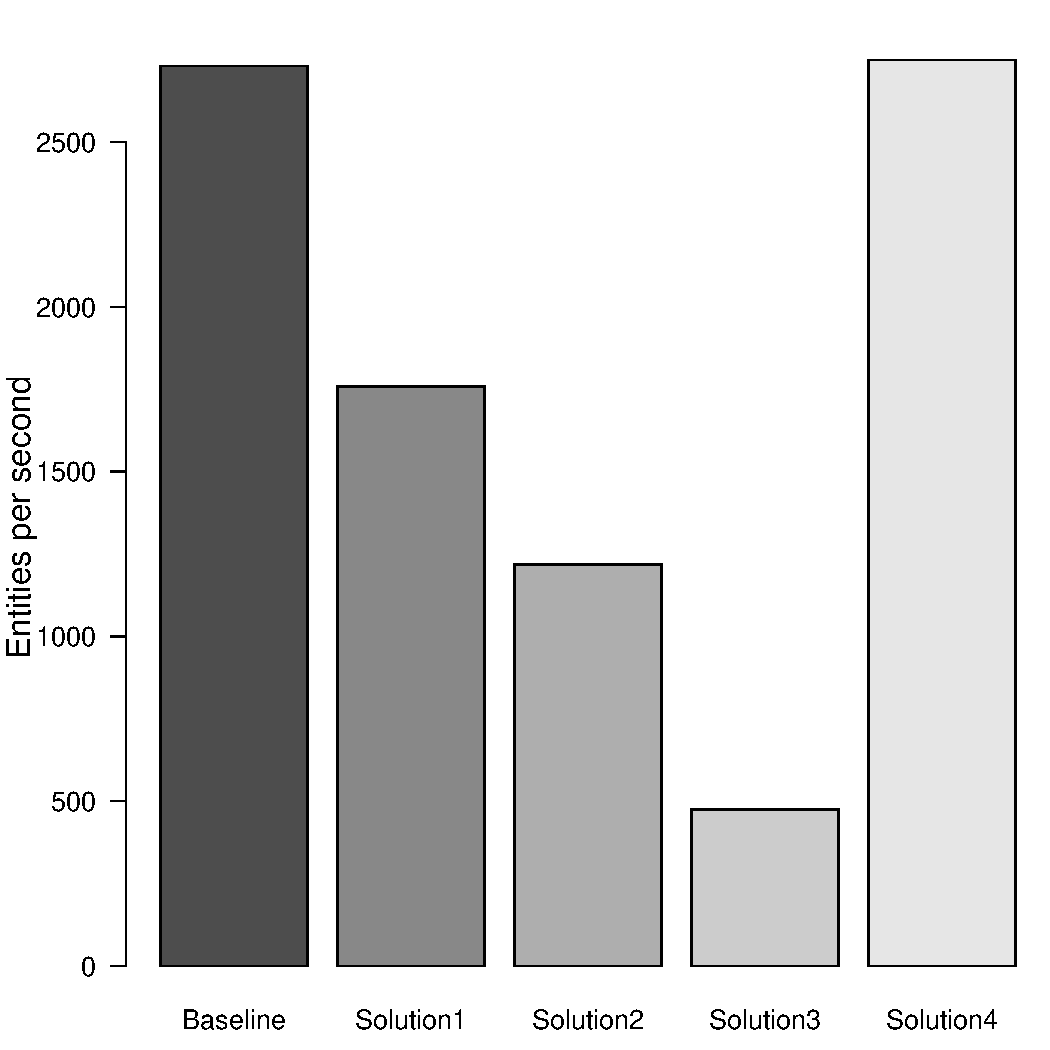
\includegraphics[width=\W]{figure/result/barplot-insert_student-tp.pdf}}
			\caption{Performance inserting students}\label{fres:insert-user}
% 		\end{figure}
% \newpage
% 	\subsection{Course}
% 		\begin{figure}[H]
			\subfigure[Response time for Insert on Course]
			{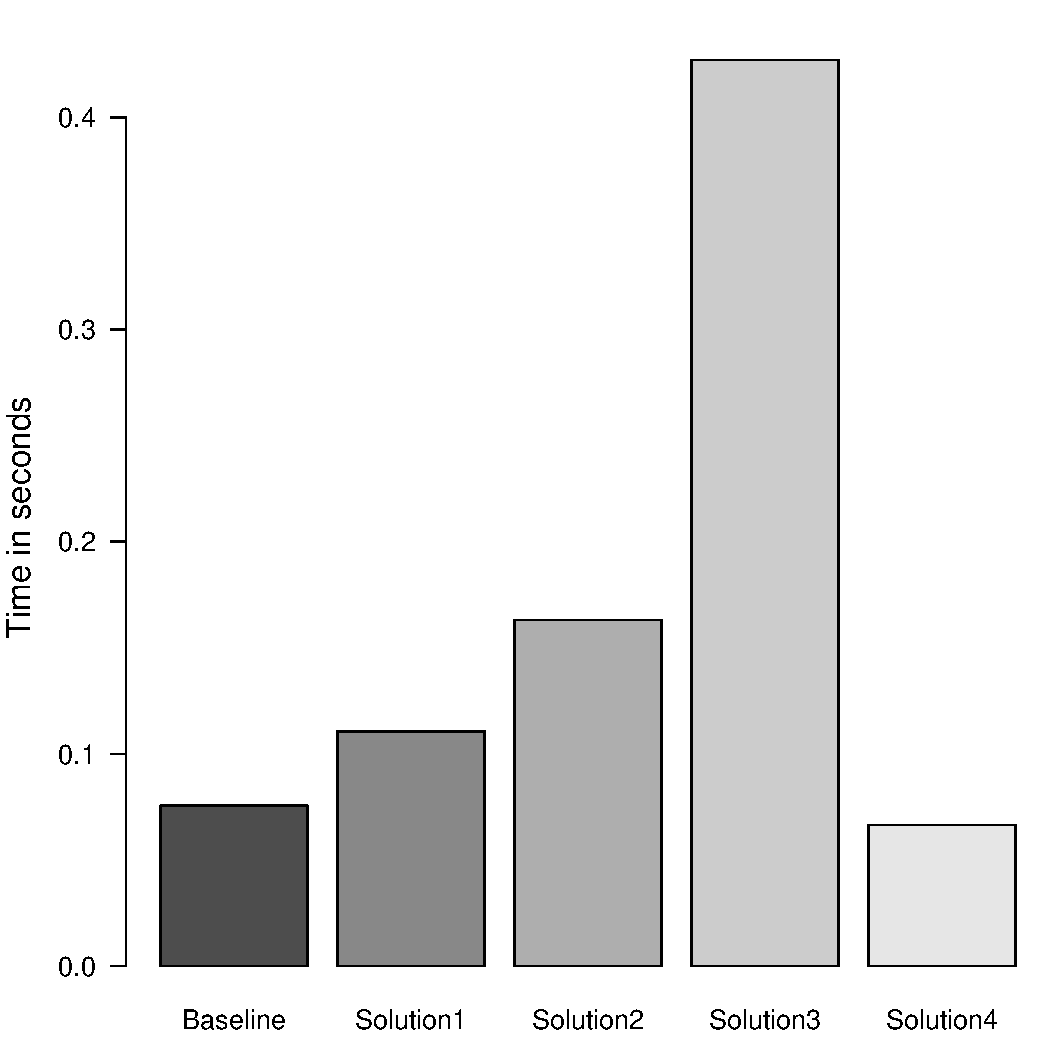
\includegraphics[width=\W]{figure/result/barplot-insert_course-rt.pdf}}
			\subfigure[Throughput for Insert on Course]
			{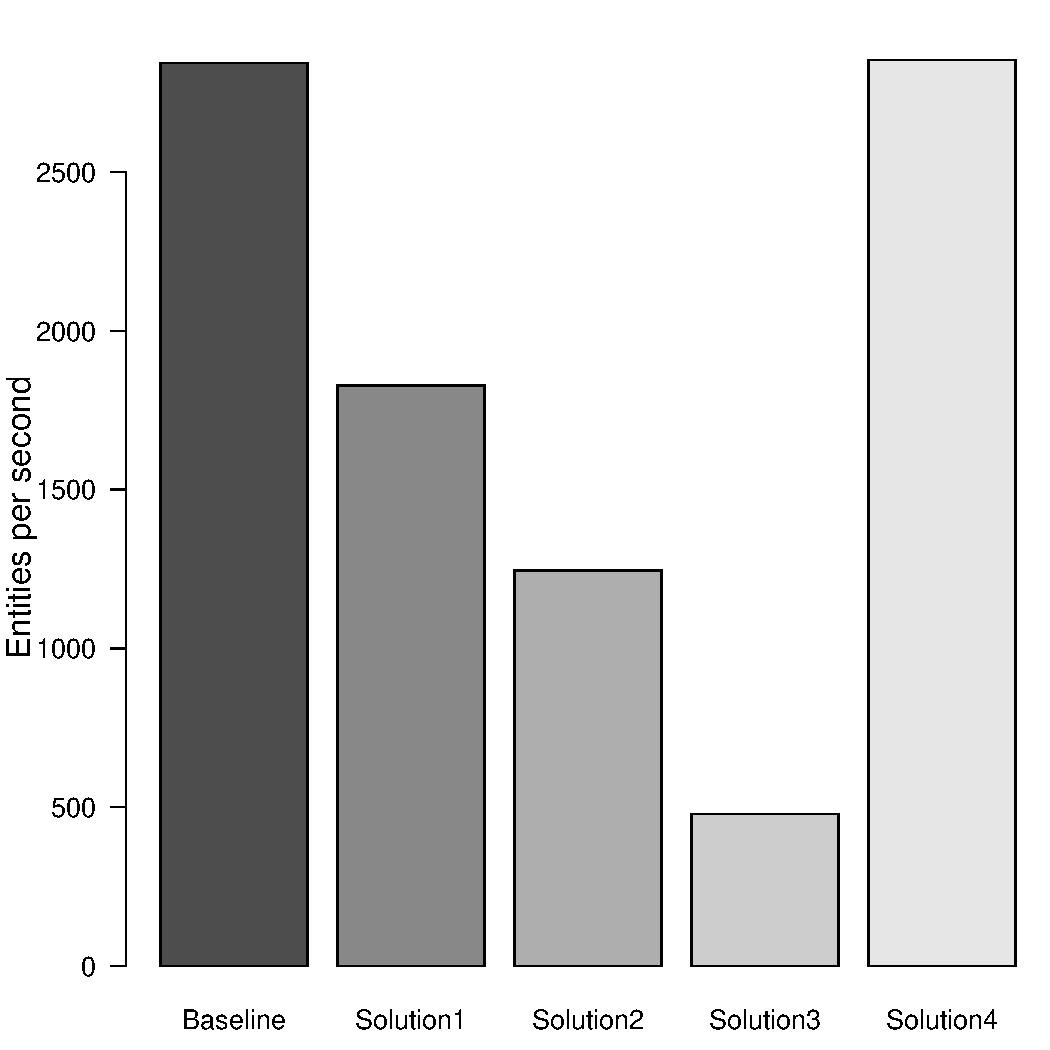
\includegraphics[width=\W]{figure/result/barplot-insert_course-tp.pdf}}
			\caption{Performance inserting courses}\label{fres:insert-course}
% 		\end{figure}
% \newpage
% 	\subsection{Enrolment}
% 		\begin{figure}[H]
			\subfigure[Response time for Insert on Enrolment]
			{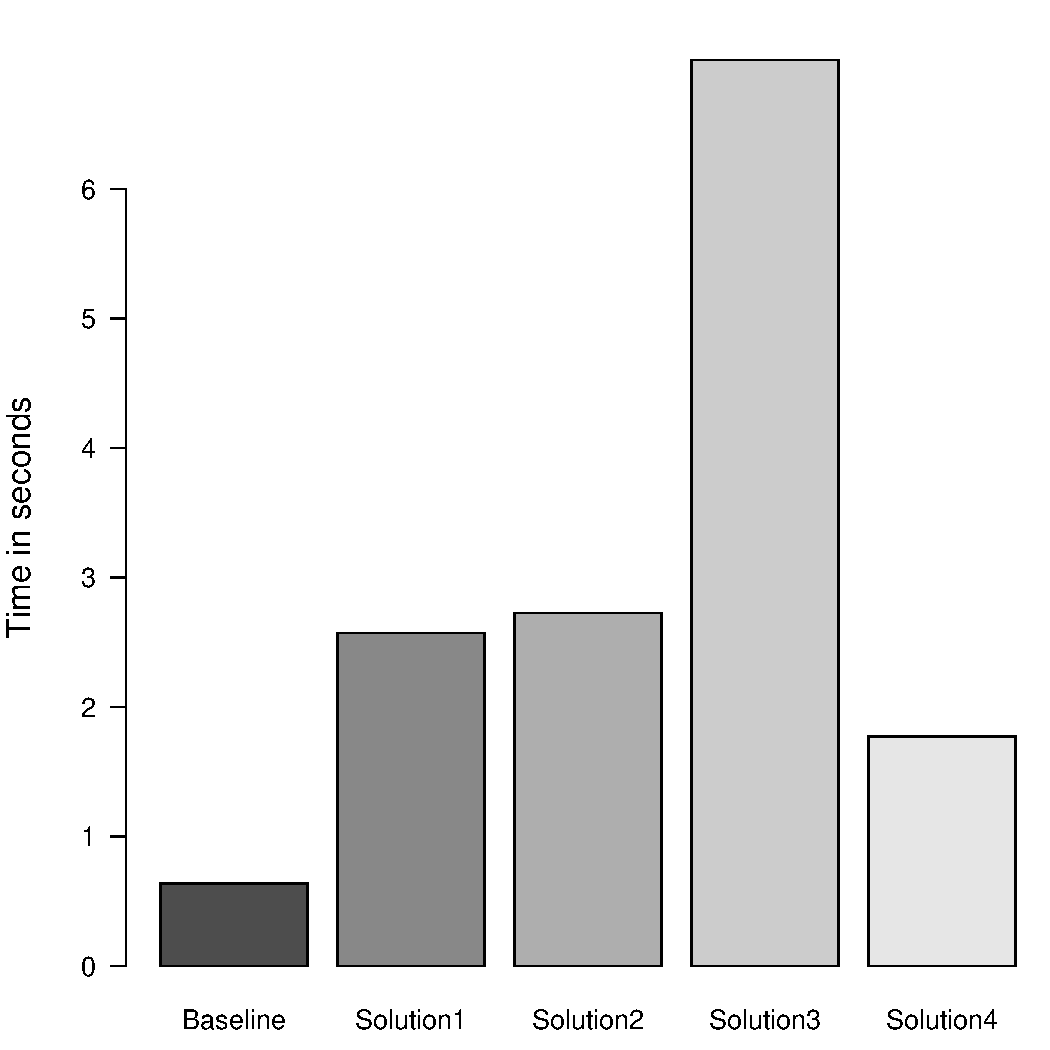
\includegraphics[width=\W]{figure/result/barplot-insert_enrolment-rt.pdf}}
			\subfigure[Throughput for Insert on Enrolment]
			{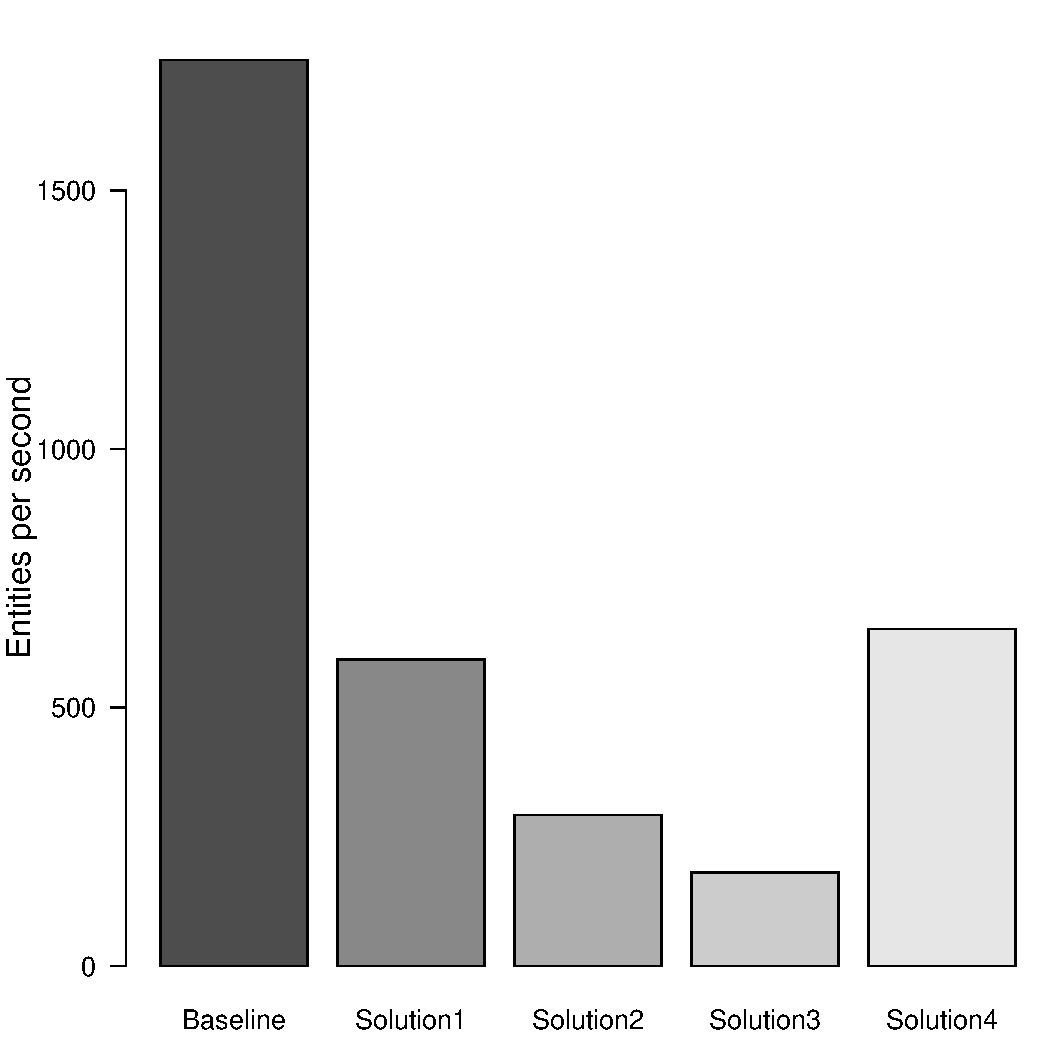
\includegraphics[width=\W]{figure/result/barplot-insert_enrolment-tp.pdf}}
			\caption{Performance inserting enrolments}\label{fres:insert-enrolment}
		\end{figure} 
%ब 

\section{Update} \label{s:results-update}
In all the solutions, the \texttt{update} operation triggers a referential
integrity validation whenever any entity of \texttt{Student}, \texttt{Course}
and \texttt{Enrolment} is updated with new values. Figure~\ref{fres:Update}
presents the results of a single update on each entity for all the solutions.
Figure~\ref{fres:Update-responsetime} shows the time taken to compete the
\texttt{update} on each entity in the solutions and
Figure~\ref{fres:Update-throughput} presents the throughput of this operation.

	\begin{figure}[H] 
		\subfigure[Response time for Update operation]
		{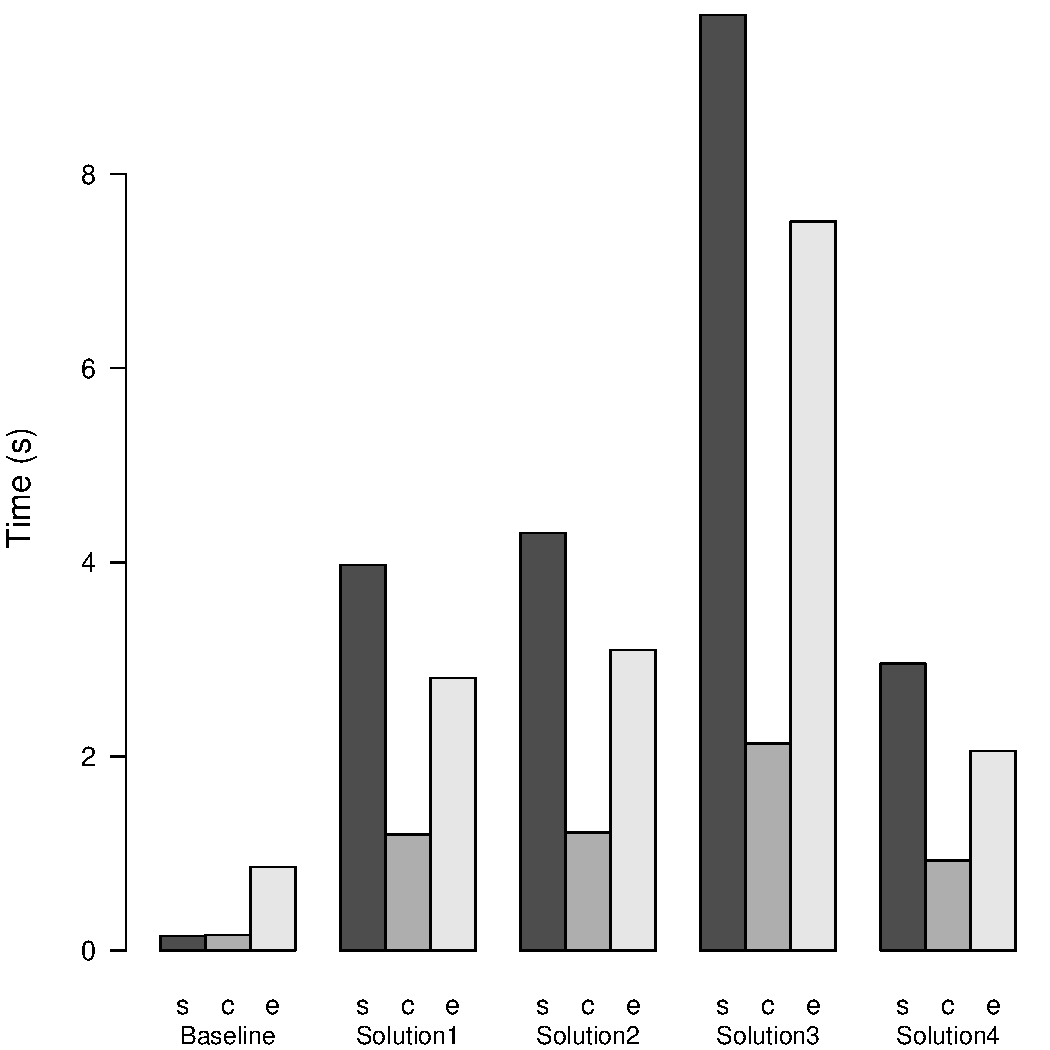
\includegraphics[width=\Width]{figure/result/barplot-update-rt.pdf}\label{fres:Update-responsetime}}
		\subfigure[Throughput for Update operation]
		{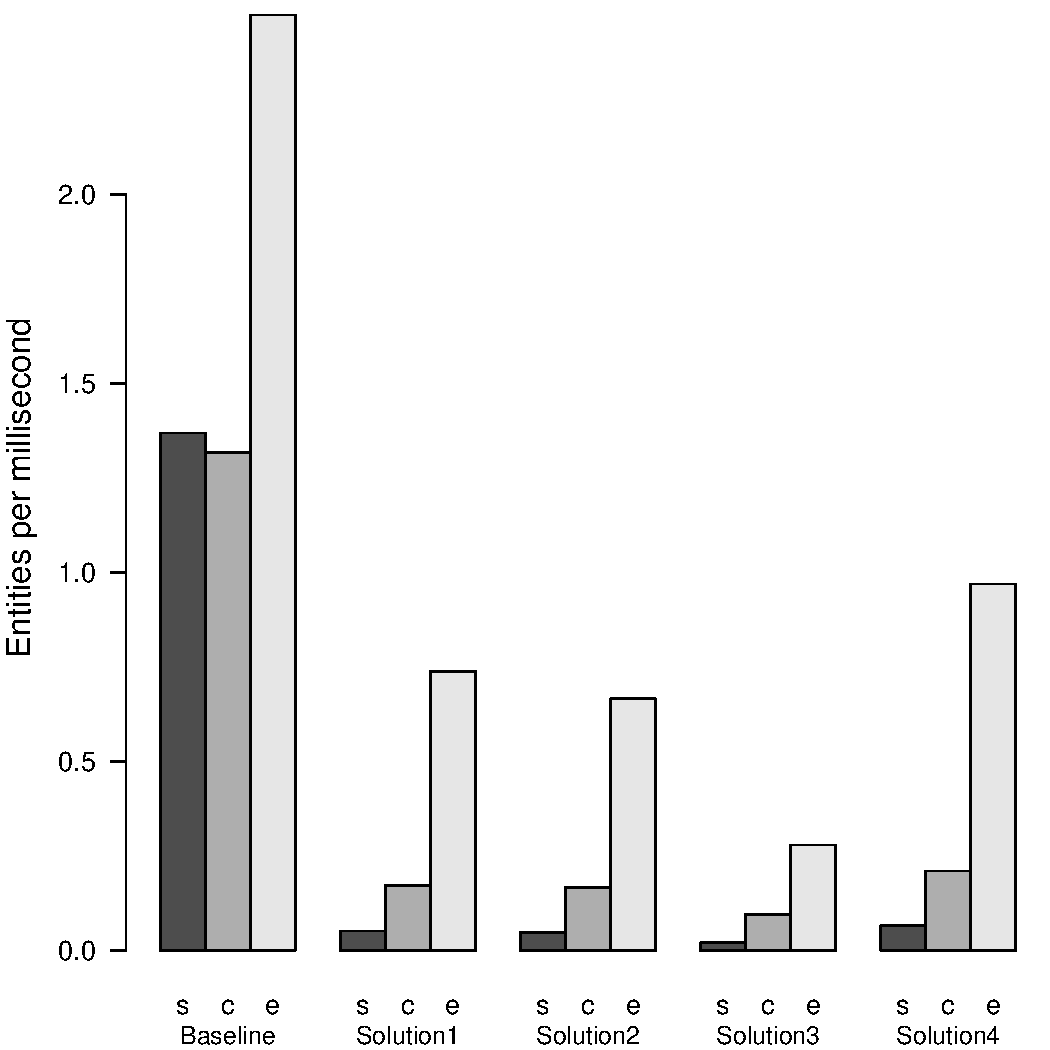
\includegraphics[width=\Width]{figure/result/barplot-update-tp.pdf}\label{fres:Update-throughput}}
		\caption{Performance of Solutions in Update}\label{fres:Update}
	\end{figure}
 
It can be seen from the results that the
\texttt{update} on \texttt{Enrolment} is the fastest in all the solutions, when
compared to \texttt{update} on other entities. On the contrary, \texttt{update}
on a \texttt{Student} entity takes the most time in all the solutions.
\texttt{update} on a \texttt{Course} entity always takes more time than
\texttt{update} on \texttt{Enrolment} but is faster than updating
\texttt{Student} entities.

These differences in the performance of an \texttt{update} on the three entities
is because of the referential integrity rules that are applied during
validation.
% which causes \texttt{update} on parent entities take more time than updating
% child entities.
Updating \texttt{Enrolment} is fastest since it involves only identifying
relevant \ac{FK} constraints in the list of constraints and then accessing the
parent column families \texttt{Student} and \texttt{Course} to verify if the new
foreign key values exist or not. After this, the new values are written to only
the \texttt{Enrolment} column family. 

However, updating a \texttt{Student} entity takes the most time since it is
a cascaded operation. After accessing its relevant \ac{FK} constraints, its
child dependencies are retrieved from \texttt{Enrolment} and updated with the new
value for the \texttt{StudentId}. This means that an \texttt{update}
accesses the metadata as well as the child column family and causes writes not
only in \texttt{Student} but also in the child column family \texttt{Enrolment}.
\texttt{update} on \texttt{Course} entities take lesser time than this because
its not a cascaded operation as the \texttt{DeleteRule} for \texttt{Course}
entities is \texttt{NoDelete}. Thus, exceptions are raised each time an
\texttt{update} is performed on \texttt{Course} entities, which means that the
response time includes measuring the time for validation as well as raising
exceptions. But this is slower than \texttt{update} on \texttt{Enrolment}
because it involves accessing the \texttt{Enrolment} column family
to identify existing child dependencies. Since these child dependencies exist
when the experiments are run, the exceptions are raised each time.

% The time involved for an \texttt{update} on a \texttt{Course} entity is  more as
% seen in Figures~\ref{fres:Update} and~\ref{fres:update-course}. In this
% operation the relevant \texttt{FK} constraints and child dependencies of the
% \texttt{Course} entity are identified and its  relevant \texttt{DeleteRule}
% is also determined.
% Since the \texttt{DeleteRule} for \texttt{Course} entities is \texttt{NoDelete}
% an exception is raised. Moreover, \texttt{Enrolment} column family is accessed
% to identify existing child dependencies. These additional operations and the
% exceptions raised make \texttt{update} on \texttt{Course} consume more time to
% complete.
% 
% The results in Figures~\ref{fres:Update} and~\ref{fres:update-user} show that
% updating a \texttt{Student} entity takes the most time in all the solutions.
% The relevant \ac{FK} constraints are accessed for this entity and
% its child dependencies are identified from \texttt{Enrolment}, which is similar
% to \texttt{update} on \texttt{course} entities. However, update on a
% \texttt{Student} entity is cascaded and involves updating all the child
% dependencies in \texttt{Enrolment} column family. This means that an
% \texttt{update} causes writes not only in \texttt{Student} but also in the child
% column family \texttt{Enrolment}. 
Note that \texttt{update} on \texttt{Student} entities causes values in
two column families to be updated, while in \texttt{Enrolment} values are
updated in only one column family and in \texttt{Course} no values are updated. 


Further details of the performance of each solution when an
\texttt{update} operation is executed on each entity is presented in 
Figures~\ref{fres:update-user},~\ref{fres:update-course}
and~\ref{fres:update-enrolment}.
% These figures show the response time to
% complete one \texttt{update} on all the three entities in every solution and
% the throughput of the operation.
Figure~\ref{fres:update-user} presents the results for an \texttt{update} on a
single \texttt{Student} entity in all the solutions and
Figures~\ref{fres:update-course} and~\ref{fres:update-enrolment} show the
performance of an \texttt{update} on a \texttt{Course} and \texttt{Enrolment}
entity in the solutions. These results show that Solution~4 is the fastest
amongst all the solutions, while Solution~3 is the slowest.
Solutions~1 and 2 perform almost similarly although the additional search for
the top row in Solution~2 makes it just slightly slower than Solution~1.
Note that in Solution~3 the \texttt{Metadata} column family is accessed multiple
times in each validation making it the slowest. Multiple accesses are needed in
order to first retrieve the relevant \ac{FK} constraints and then to retrieve
information about the child or parent entities. Although Solution~4 stores
metadata separately like Solution~3, it caches the \texttt{Metadata} column
family and reuses the cache to avoid such multiple accesses to the column
family.

When compared to the baseline, the \texttt{update} operation on all the
entities take considerably more time in all the solutions because of
their different metadata storage designs. The validations and metadata access
for parent entities make Solution~4 20 times slower than the baseline and
Solution~3 almost 60 times slower in cascaded updates, which is the most
time consuming \texttt{update}. 
Solutions~1 and 2 are almost more than 25 times slower than
baseline in such updates. However, updates on child entities make Solution~4
only slightly slower than the baseline while Solution~3 is three times slower.
In such cases, Solution~1 and 2 are almost 1.5 times slower than the baseline.

% Note that in all the solutions the \texttt{update} on . This is because of the different
% referential integrity rules applied on the entities. 
 
\begin{landscape}
		\begin{figure}
		\centering
		\newcommand{\W}{.4\textwidth}
			\subfigure[ Update on Student]
			{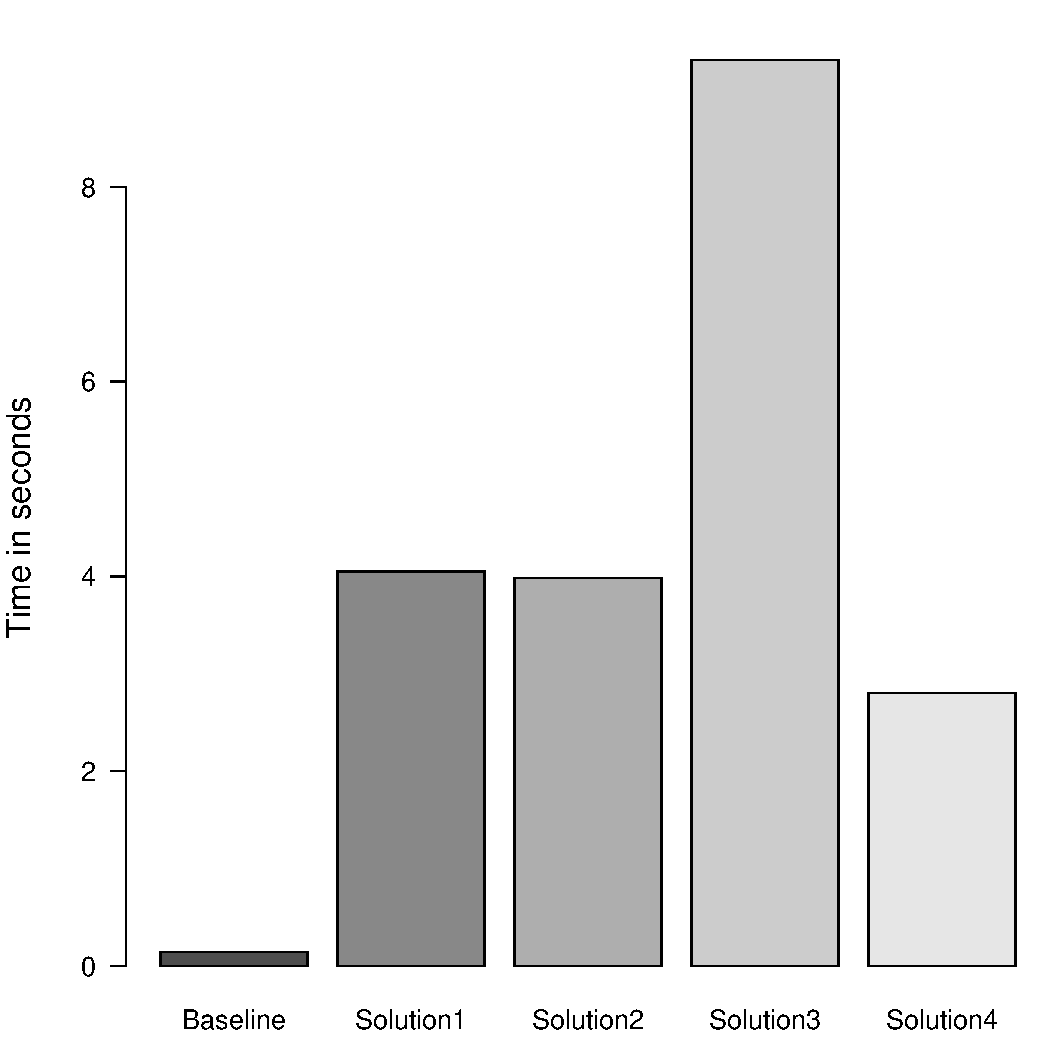
\includegraphics[width=\W]{figure/result/barplot-update_student-rt.pdf}}
			\subfigure[ Update on Course]
			{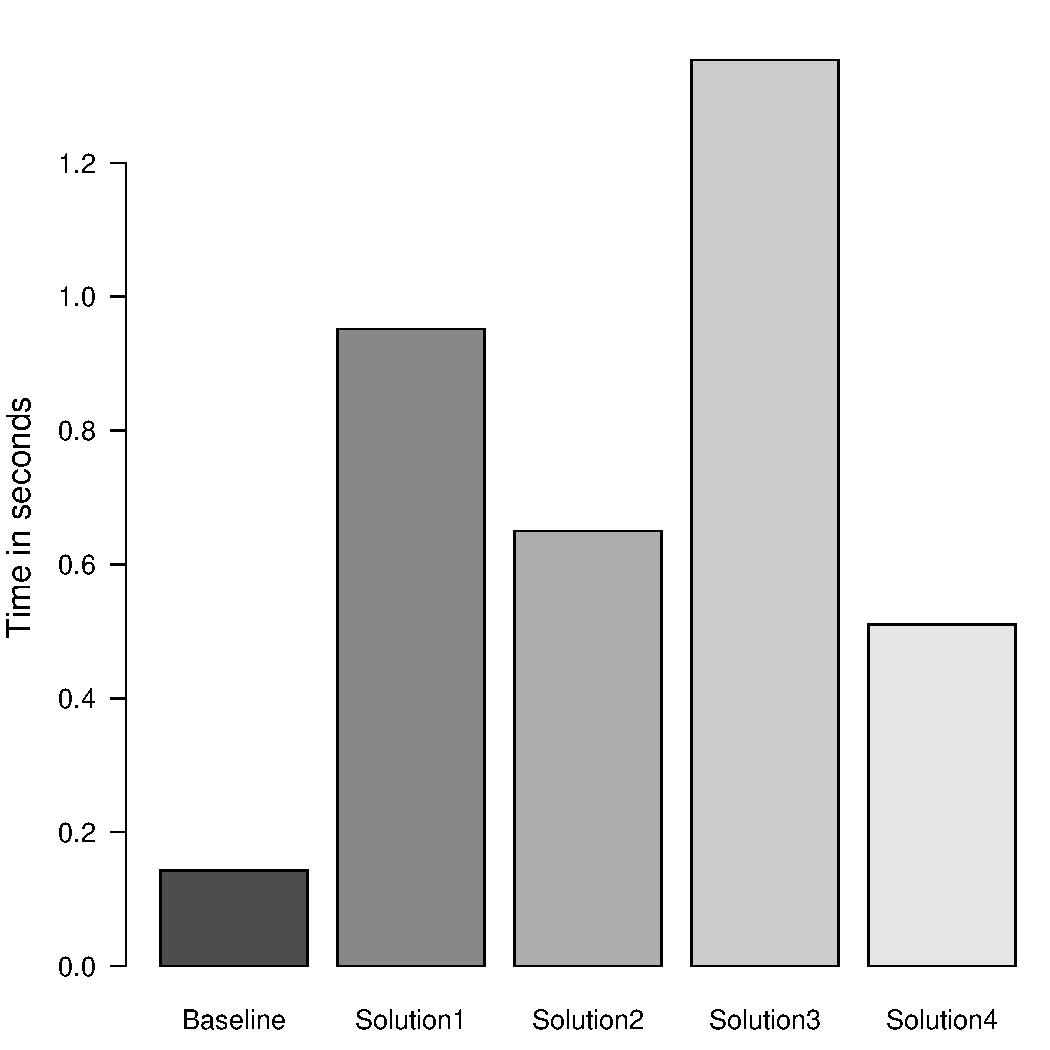
\includegraphics[width=\W]{figure/result/barplot-update_course-rt.pdf}}
			\subfigure[ Update on Enrolment]
			{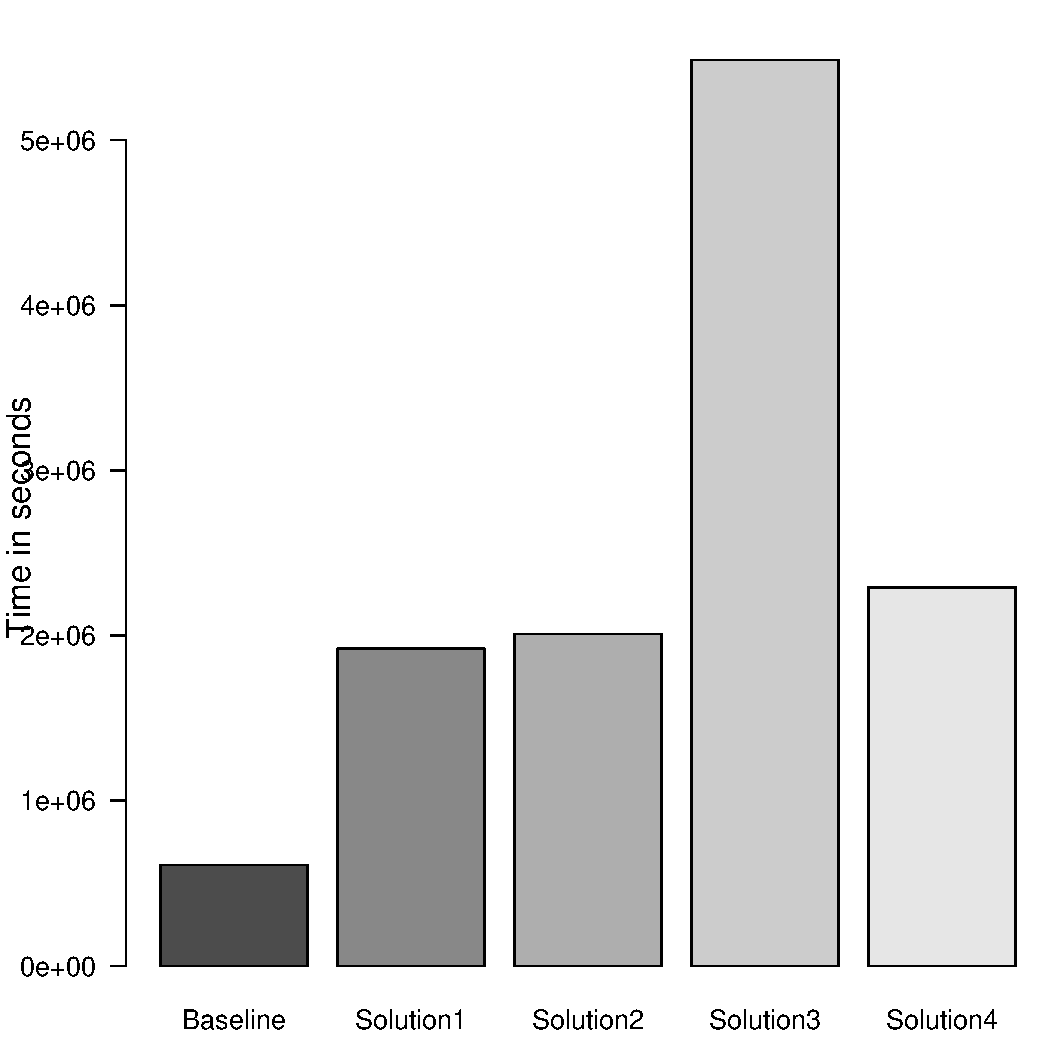
\includegraphics[width=\W]{figure/result/barplot-update_enrolment-rt.pdf}}
			\caption{Response time updating entities}\label{fres:update-response-time}
			
			\subfigure[Update on Student]
			{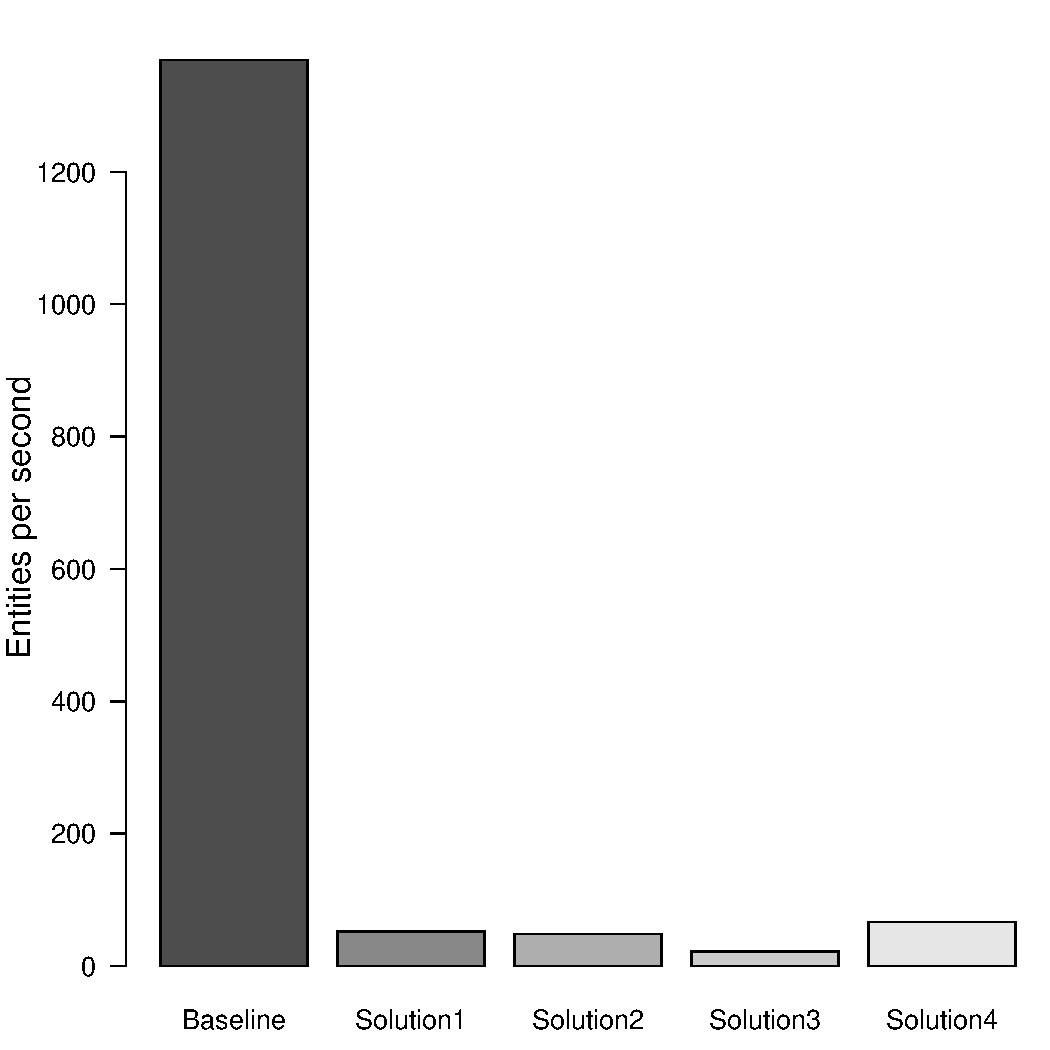
\includegraphics[width=\W]{figure/result/barplot-update_student-tp.pdf}}			
			\subfigure[ Update on Course]
			{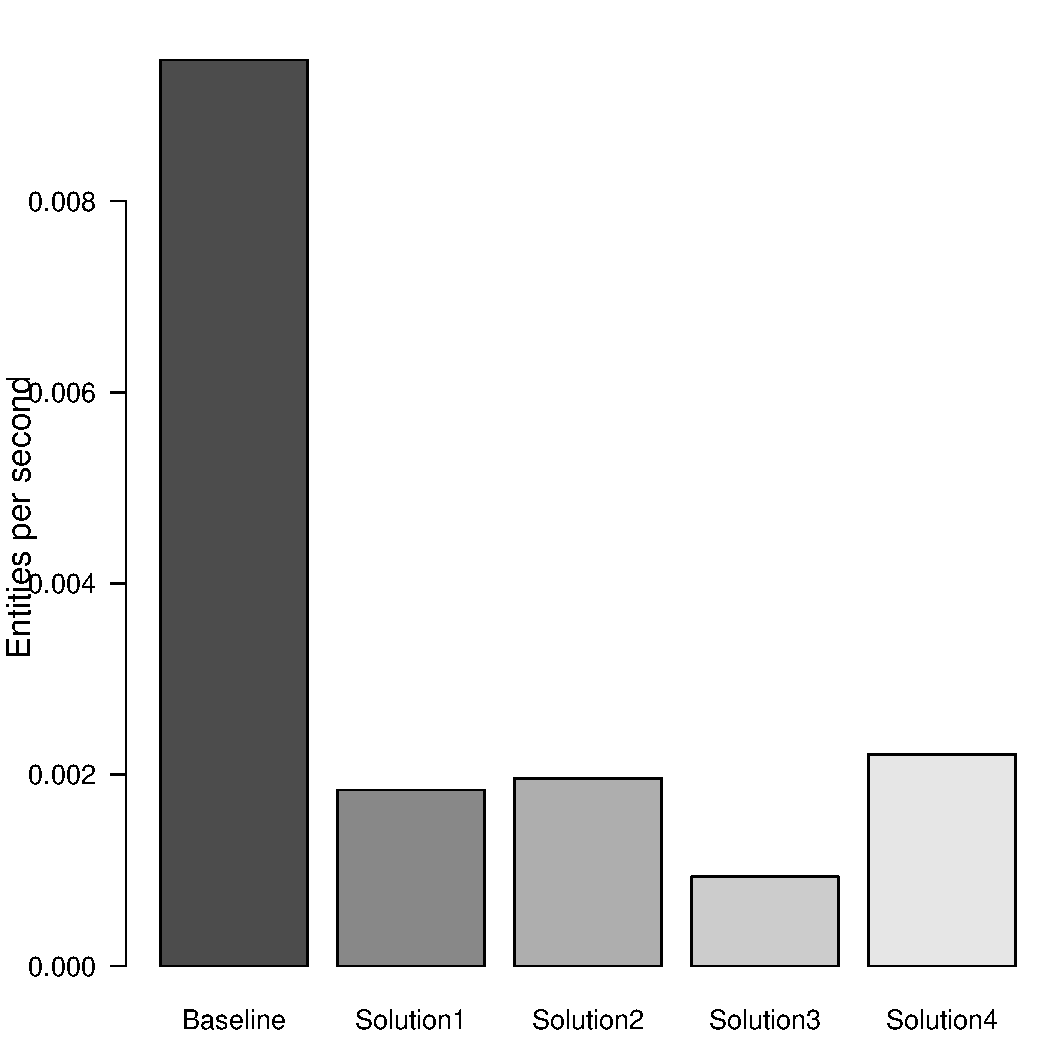
\includegraphics[width=\W]{figure/result/barplot-update_course-tp.pdf}}
			\subfigure[Update on Enrolment]
			{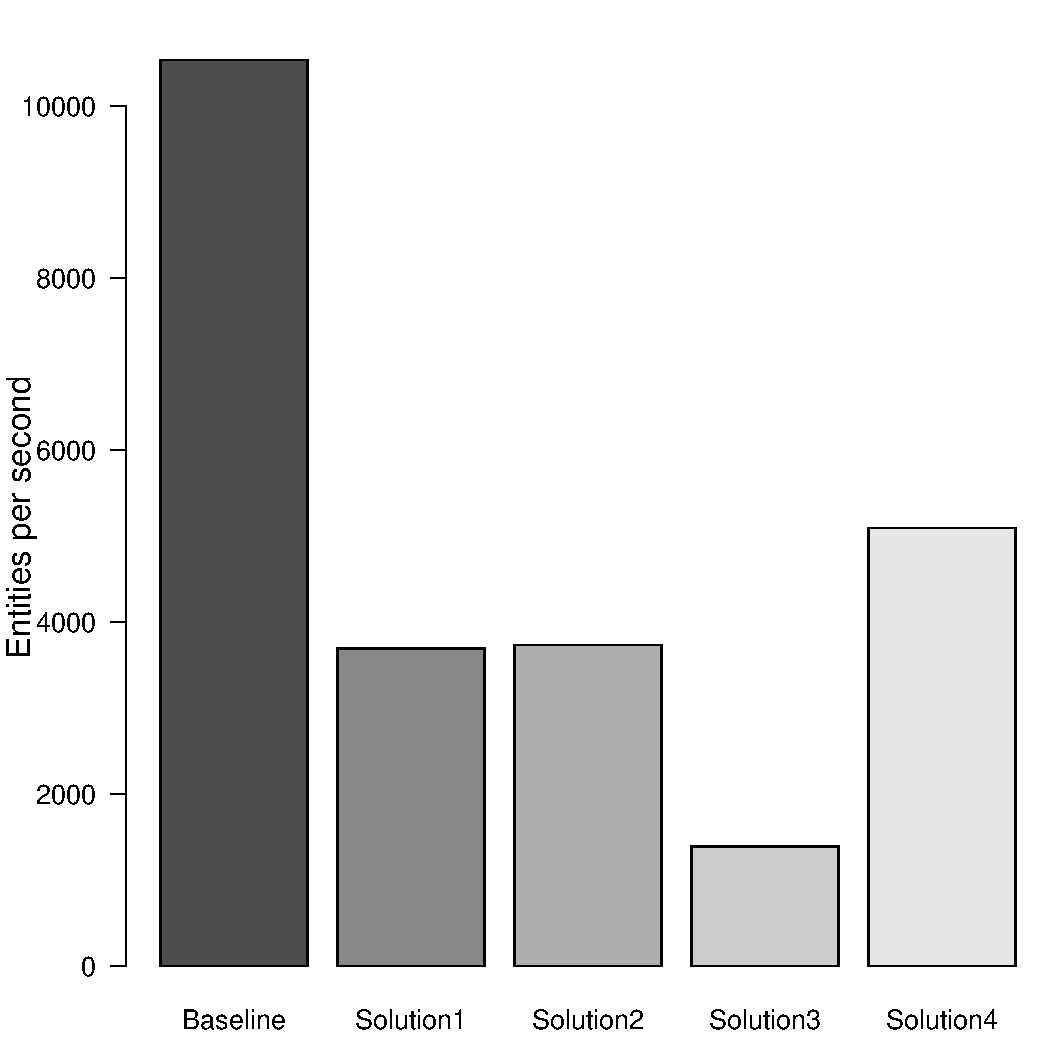
\includegraphics[width=\W]{figure/result/barplot-update_enrolment-tp.pdf}}
			\caption{Throughput updating entities}\label{fres:update-throughput}
		\end{figure}
\end{landscape}
%ब 
\section{Delete} \label{s:results-Delete}

The \texttt{delete} operation triggers referential integrity validations
whenever entities are deleted in the experiments.
Figure~\ref{fres:Delete} presents the results of the \texttt{delete} operation
on each entity for all the solutions.
Specifically, Figure~\ref{fres:Delete-responsetime} shows the average
response time to perform a single \texttt{delete} on each entity in the
solutions and Figure~\ref{fres:Delete-throughput} presents the
respective throughput for this operation.

	\begin{figure}[H] 
	\newcommand{\W}{.5\textwidth}
		\subfigure[Response time for Update operation]
		{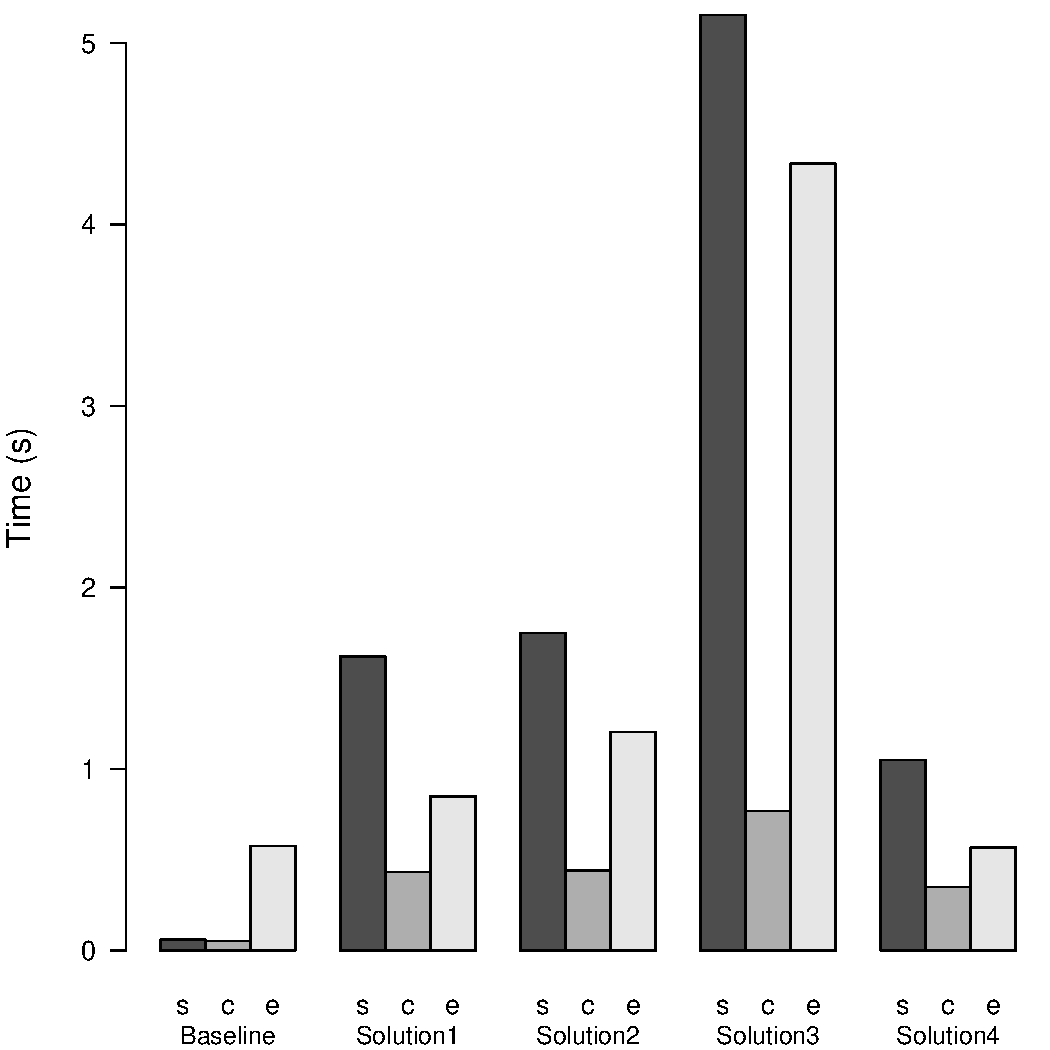
\includegraphics[width=\W]{figure/result/barplot-delete-rt.pdf} \label{fres:delete-}\label{fres:Delete-responsetime}}
		\subfigure[Throughput for Update operation]
		{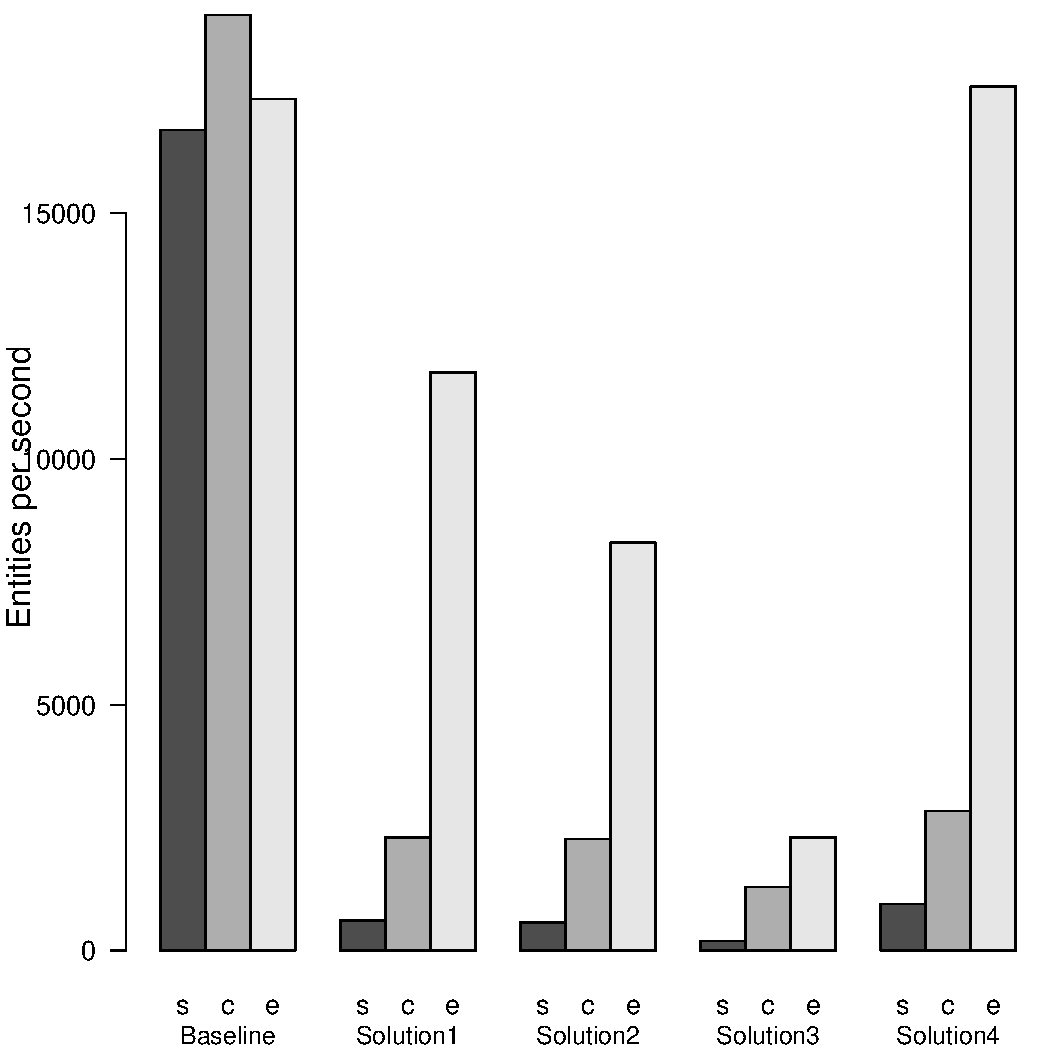
\includegraphics[width=\W]{figure/result/barplot-delete-tp.pdf} \label{fres:delete-}\label{fres:Delete-throughput}}
		\caption{Performance of Solutions in Update}\label{fres:Delete}
	\end{figure}
 
As seen in  the results, the \texttt{delete} in \texttt{Enrolment}
is the fastest in all the solutions, while  \texttt{delete} in
\texttt{Student} is the slowest. The \texttt{delete} operation on 
\texttt{Course} is faster than deleting \texttt{Student} entities but it
always takes more time than \texttt{delete} in \texttt{Enrolment}.

As seen in \texttt{update}, the difference in  performance of the operation
on the different entities is because of the referential integrity rules on
child and parent entities. Deleting \texttt{Enrolment} entities is faster as it 
does not invoke any referential integrity validations since \texttt{Enrolment}
has no child dependencies in it.
However, this operation is  slower than the baseline in all the solutions
because it involves accessing metadata to retrieve the relevant constraints of
\texttt{Enrolment} in order to determine if any child dependencies exist or
not.

Deleting \texttt{Student} entities is a cascaded operation which involves
deleting the child dependencies in the \texttt{Enrolment} column family. This
operation is slower because  the relevant constraints need to be  accessed and
the child entities in \texttt{Enrolment}  that have a reference to the
\texttt{Student} have to be deleted. 

Similarly, \texttt{delete} on \texttt{Course} entities also involves accessing
the relevant constraints and finding the child dependencies in
\texttt{Enrolment}. However, in the experiments,  all the entities in
\texttt{Enrolment} are already deleted before \texttt{delete} is invoked on
\texttt{Course} entities. Hence, \texttt{delete} in \texttt{Course} actually
deletes the entities as there are no existing child dependencies.
Notice that \texttt{delete} on \texttt{Course} involves the time to access
metadata as well as \texttt{Enrolment} in order to search for any existing child
dependencies and values are deleted from a single column family. However,
\texttt{delete} on \texttt{Student} entities involve deleting values from two
column families (\texttt{Student} and \texttt{Enrolment}). This
makes \texttt{delete} in \texttt{Course} faster than \texttt{delete} in
\texttt{Student}.

Finally, Figures~\ref{fres:delete-response-time}
and~\ref{fres:delete-throughput} show the average response time and throughput
of \texttt{delete} on all the entities. It can be seen from these results that
Solution~4 takes the least time to complete a \texttt{delete} operation on each
entity, while Solution~3 takes the most time. Since Solution~4 caches the
metadata of all the entities, it avoids multiple accesses to the
\texttt{Metadata} column family whereas Solution~3 requires accessing
\texttt{Metadata} each time a constraint has to be accessed for an entity. The
performance of Solutions~1 and 2 are comparable to each other even though
Solution~2 takes slightly more time due to its additional search operation to
locate the top row.

When compared to the baseline, all the solutions take longer to delete entities.
As mentioned previously, this is because all the solutions involve accessing
relevant constraints and performing validations.
Solutions~1 and 2 are almost 2 times slower than baseline  when
\texttt{Enrolment} entities are deleted while Solution~3 is almost 7 times
slower. Solution~4 is almost similar to the baseline in this case  which shows
that accessing the metadata does not cause much difference in the performance.


However, in a cascaded delete which includes referential integrity validations
Solutions~1 and 2 are more than 23 times slower than the
baseline while Solution~3 is almost 80
times slower. Solution~4  is up to 17 times slower than the baseline.



\begin{landscape}
		\begin{figure}
		\centering
		\newcommand{\W}{.4\textwidth}
			\subfigure[Delete on Student]
			{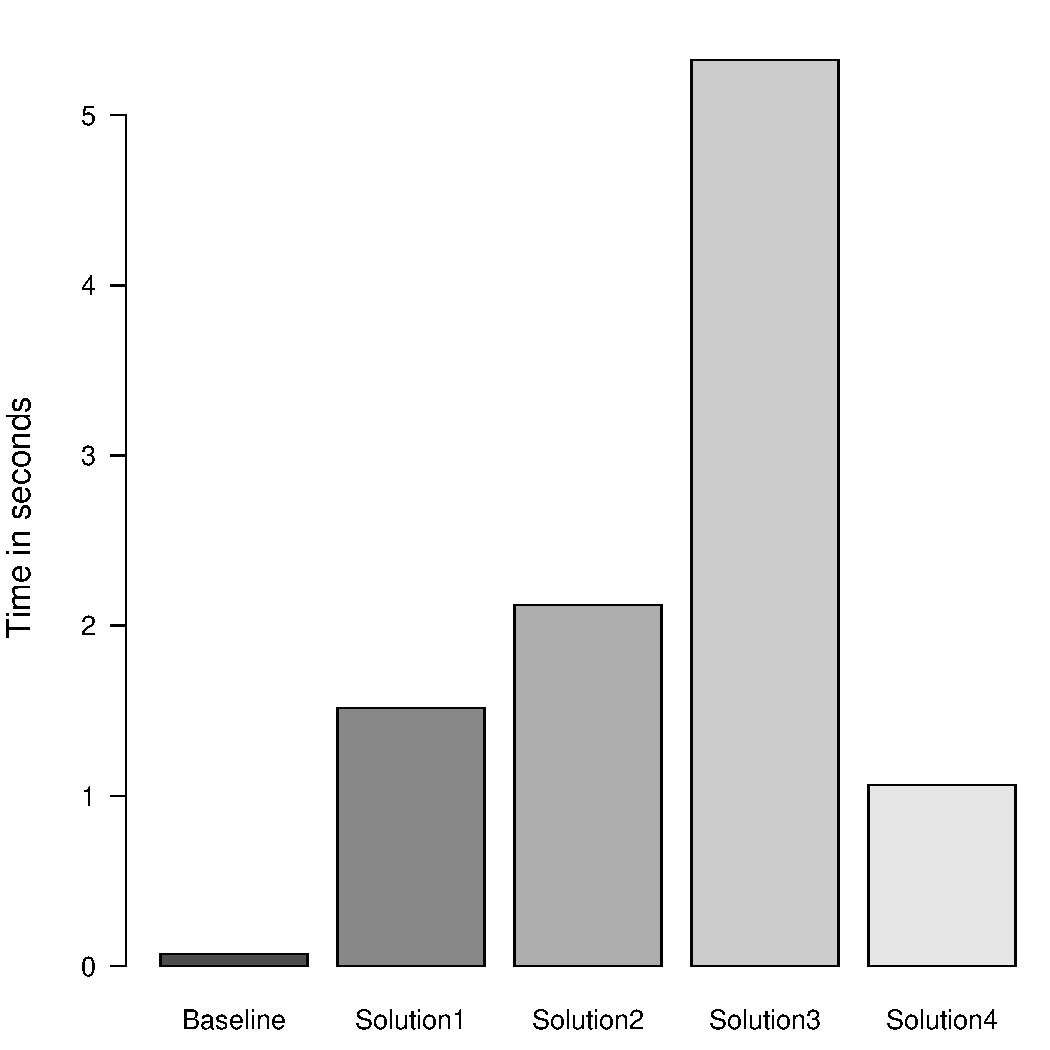
\includegraphics[width=\W]{figure/result/barplot-delete_student-rt.pdf}
			\label{fres:delete-user}}
			\subfigure[Delete on Course]
			{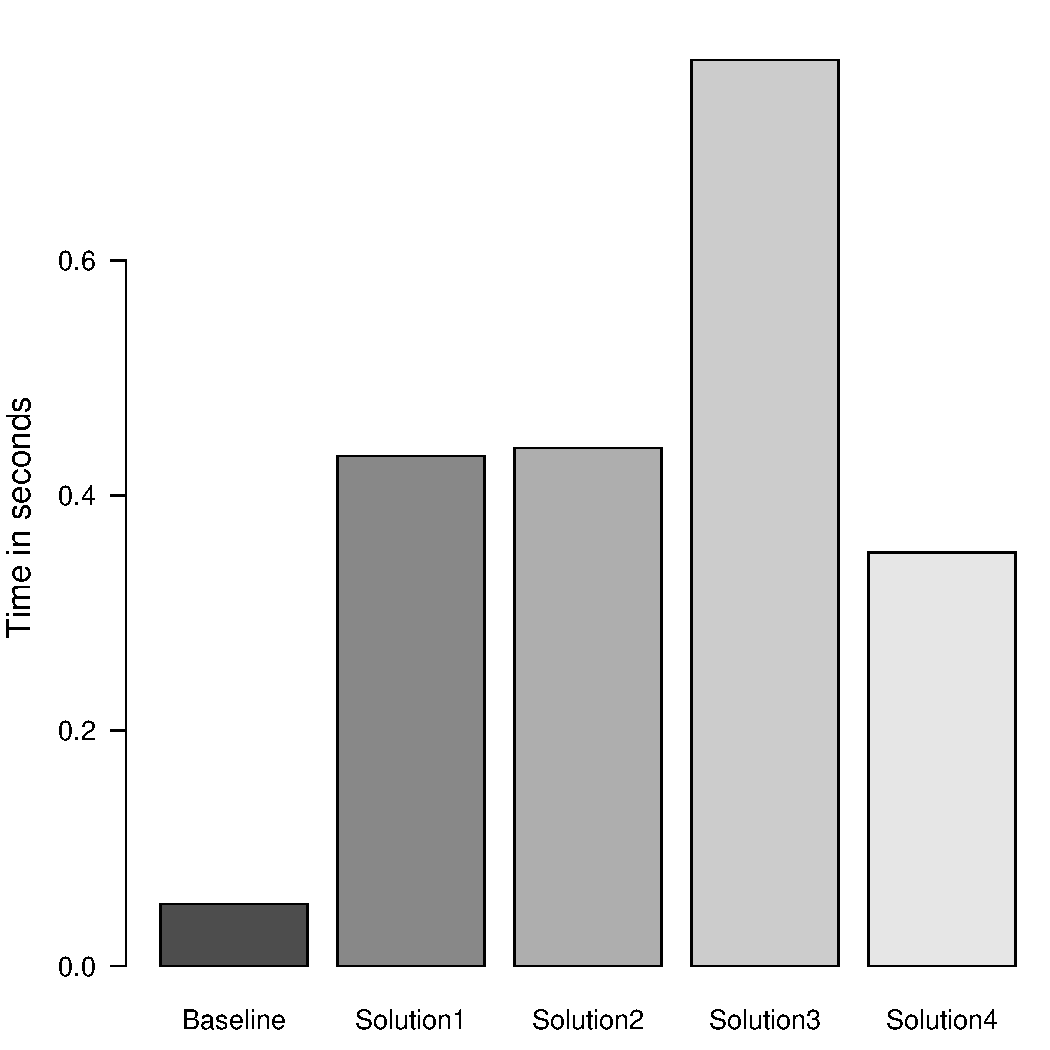
\includegraphics[width=\W]{figure/result/barplot-delete_course-rt.pdf}
			\label{fres:delete-course}}
			\subfigure[ Delete on Enrolment ]
			{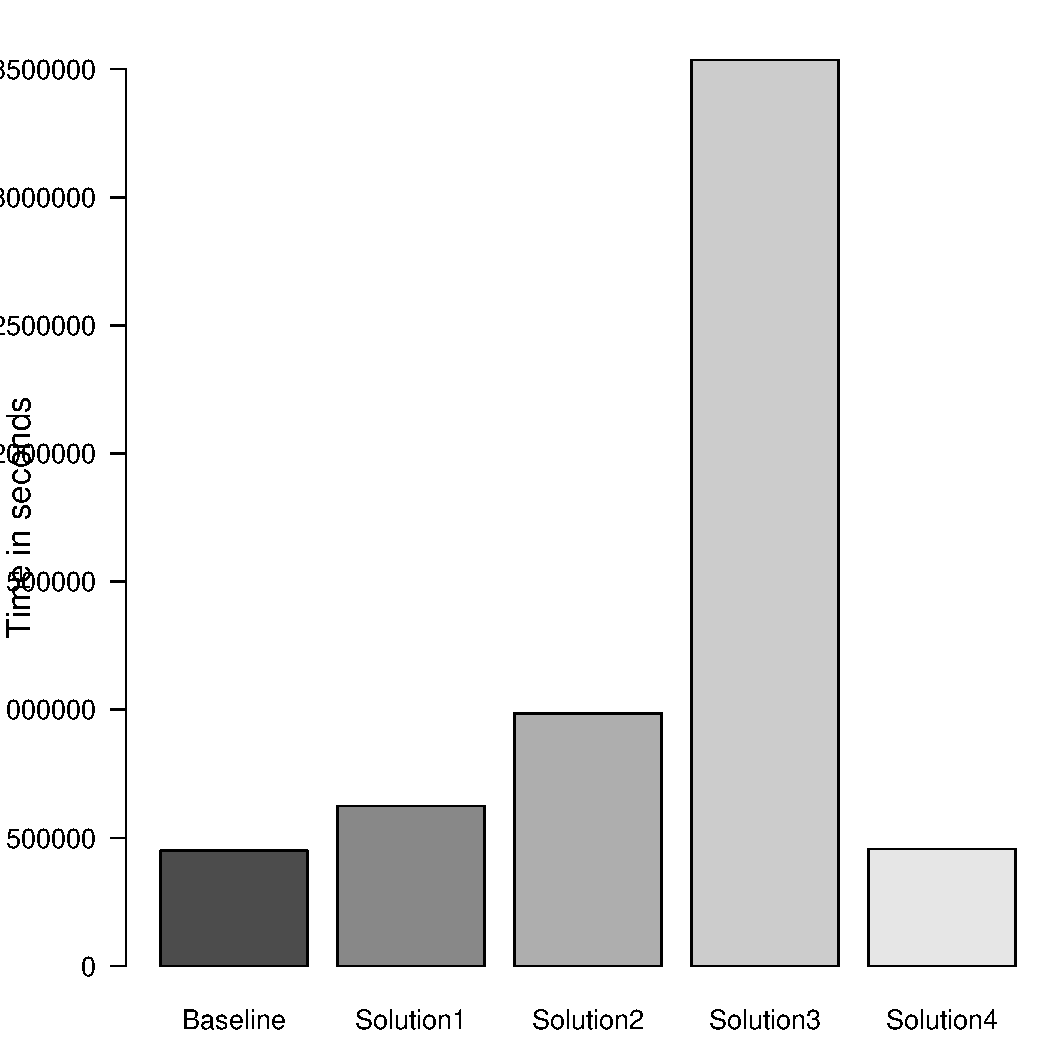
\includegraphics[width=\W]{figure/result/barplot-delete_enrolment-rt.pdf}
			\label{fres:delete-enrolment}}
			\caption{Response time deleting entities}\label{fres:delete-response-time}
						
			\subfigure[Delete on Student]
			{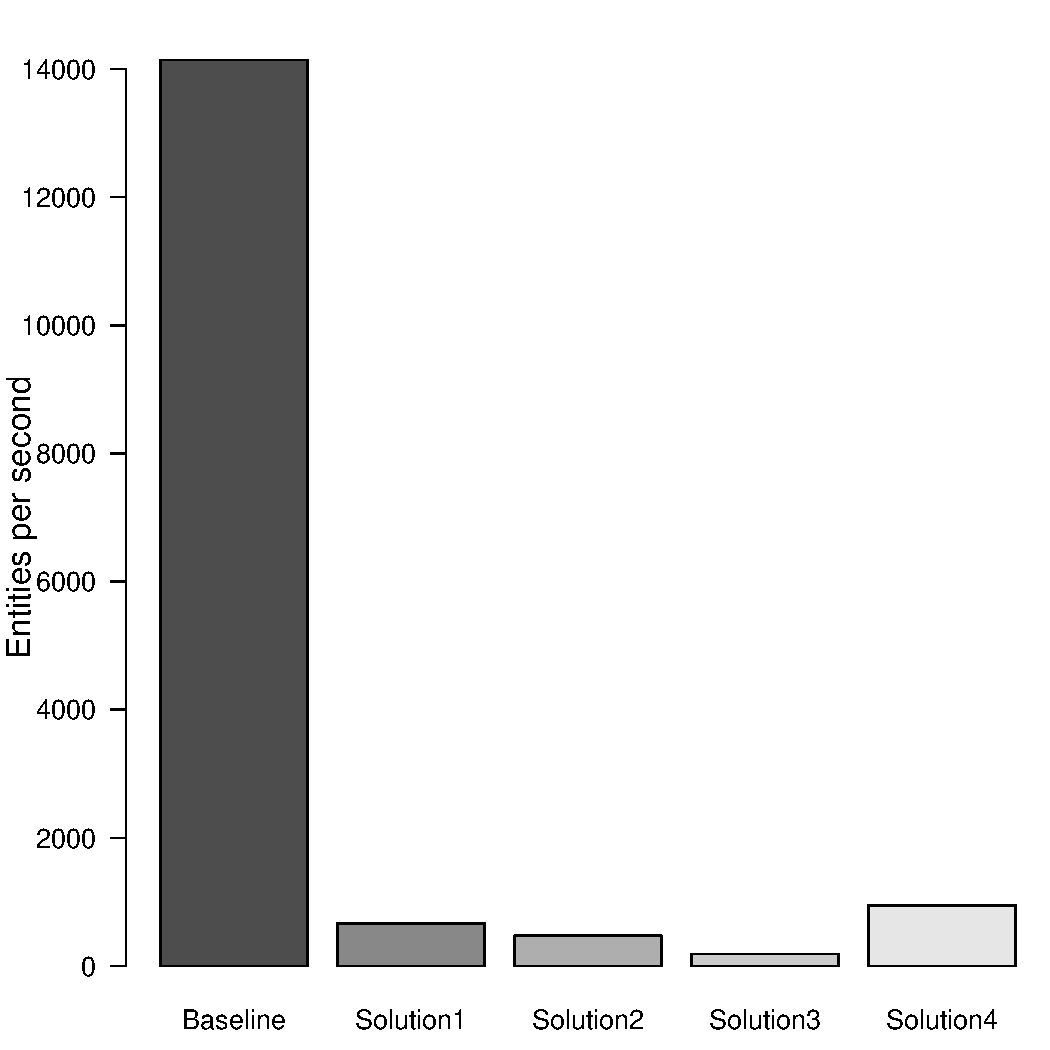
\includegraphics[width=\W]{figure/result/barplot-delete_student-tp.pdf} \label{fres:delete-}}
			\subfigure[Delete on Course]
			{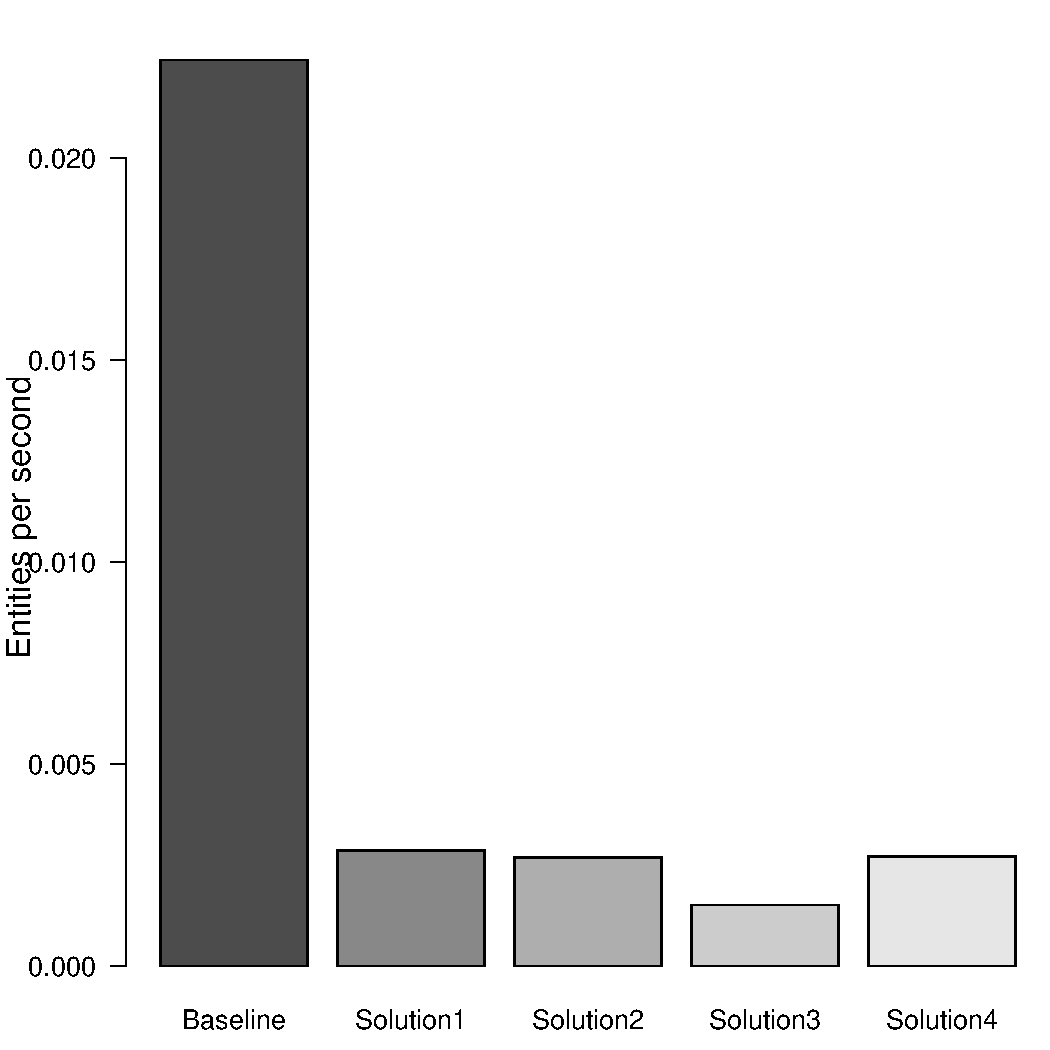
\includegraphics[width=\W]{figure/result/barplot-delete_course-tp.pdf} \label{fres:delete-}}
			\subfigure[Delete on Enrolment]
			{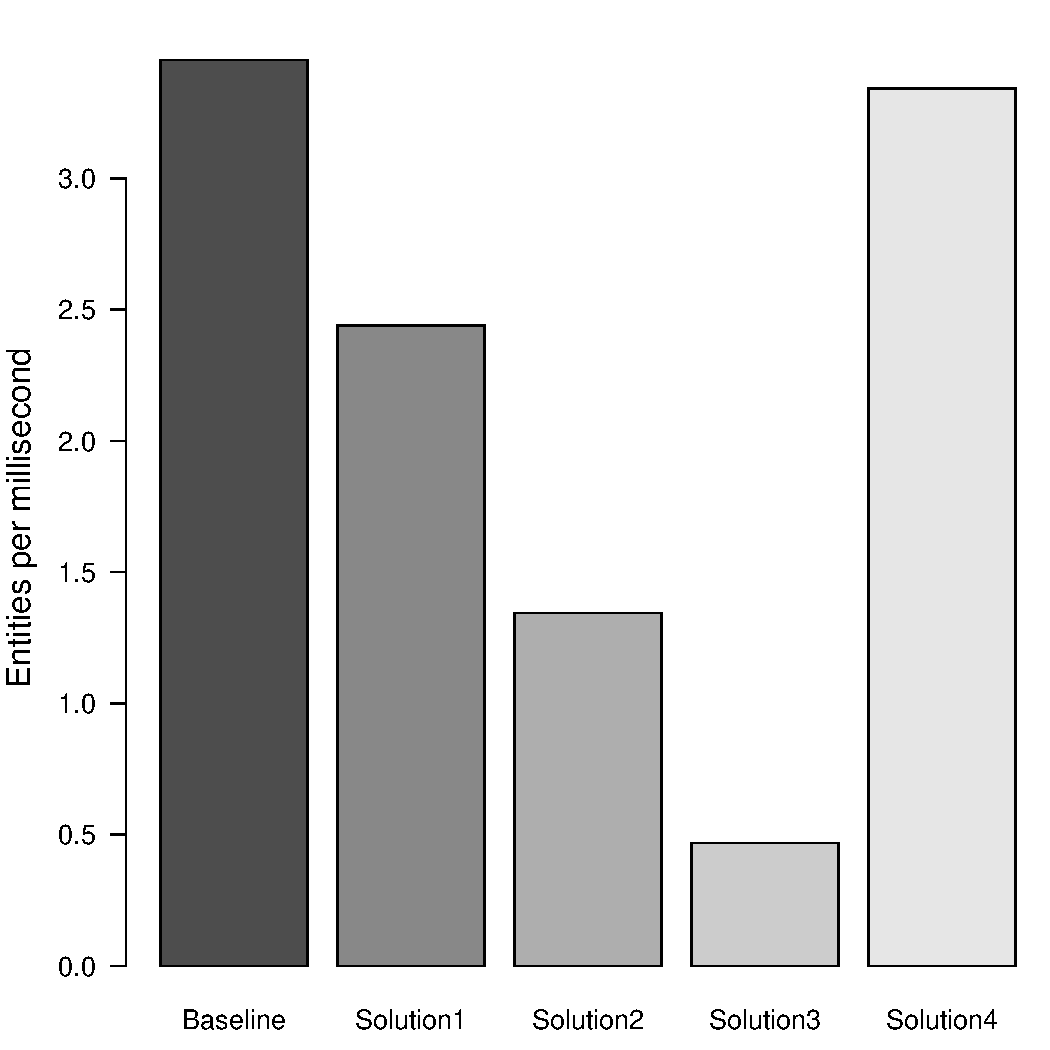
\includegraphics[width=\W]{figure/result/barplot-delete_enrolment-tp.pdf} \label{fres:delete-}}
			\caption{Throughput deleting entities}\label{fres:delete-throughput}
		\end{figure}
\end{landscape}


\section{Observations} 
From all the results and its analysis, it can be seen that the \texttt{insert}
operation takes the least time to complete when compared to \texttt{update}
\texttt{delete}. This is mainly because in \texttt{insert}, validations are
triggered on only the \texttt{Enrolment} column family. 

On the other hand, \texttt{update} takes the most time on all the entities in
every solution, mainly due to the cascaded effect of this operation which
involves accessing child column families and changing its values. Note that
\texttt{update} on \texttt{Enrolment} is similar to \texttt{insert} on
\texttt{Enrolment} because both operations involve checking whether the foriegn
keys exist in the parent column families and inserting the values. However,
\texttt{update} on \texttt{student} and  \texttt{Course} entities takes more
time than inserting these entities because \texttt{update} involves additional
searches and writes in more than one column family whereas inserting these
entities cause no validations since they have no referencing values.

\texttt{delete} is faster than \texttt{update} in all the solutions since
entities are not immediately deleted due to the tombstone effect in Cassandra.
It also does not involve more writes like the \texttt{update} operations since
values are only deleted and not written in a \texttt{delete} operation.
Moreover, deleting child entities do not cause validations while updating any
entity causes validations. When compared with the \texttt{insert} operation,
\texttt{delete} takes more time in the case of parent entities, \texttt{student}
and \texttt{course} because inserting parent entities do not cause referential
integrity validations, but inserting them does. Conversely, deleting child
entities is faster than inserting child entities since it does not trigger such
validations.

% \texttt{delete} generally consumes more
% time than \texttt{insert} in the solutions mainly because However, deleting
% \texttt{enrolment} entities involves lesser time than \texttt{insert} on these
% entities, mainly because deleting child entities do not trigger validations.
\section{Summary} \label{s:results-summary}

This chapter presented the results of the experiments that showed the response
time and throughpiut of the operation on the entities in eveyr solution. It is
learnt from the results that Solution~4 preforms the best amongst the solutions
and performs similar to the baseline when no validations are triggered.
Solution~3 performs the worst amongst the solutions and is slower than the
baseline even when validations are not triggerred because simply accessing the
metedata from a separate column family each time affects its performance.
Solutions~1 and 2 perform similarly in all the operations on the entities which
is mainly because the metadata is embedded with the entity. Solution~2 consumes
slightly more time than Solution~1 as it searches for the top row to identify
constraints on each operation. 

Analysing the results showed that amongst the operations, \texttt{insert} took
the lest time while \texttt{update} took the most time and \texttt{delete} was
faster than \texttt{insert} only in the case of child entities. These variations
were mainly due to the different referential integrity rules that are applied
on parent and child entities and the \texttt{DeleteRule} applied on these
entities.

The entities behaved differently in each operation due to the various
referential integrity rules and the data manipulation rules applied on them.
\texttt{Enrolment} being a child entity triggers validations during
\texttt{update} and \texttt{insert} operations, while \texttt{Student} and
\texttt{Course} are parent entities and trigger validations in both
\texttt{update} and \texttt{delete}. Thus parent entities are faster to operate
on in an \texttt{insert} operation, while child entities are faster only in a
\texttt{delete} operation. 
	